\documentclass[10pt]{article}

\usepackage[a4paper,margin=0.65in]{geometry}
\usepackage{amsmath,amssymb}
\usepackage{graphicx}
\usepackage{booktabs}
\usepackage{array}
\usepackage{float}
\usepackage{hyperref}
\usepackage{enumitem}
\usepackage{xcolor}
\usepackage{tikz}
\usetikzlibrary{positioning,arrows.meta,shapes.geometric}

\setlist{nosep,leftmargin=*}
\renewcommand{\arraystretch}{1.2}
\setlength{\parindent}{0pt}
\setlength{\parskip}{2pt}

\tikzset{
layer/.style={
draw,
rounded corners,
minimum width=1.5cm,
minimum height=0.6cm,
align=center,
fill=blue!10,
font=\scriptsize
},
arrow/.style={
-{Latex[length=2mm]},
thin
}
}

\begin{document}

%%%%%%%%%%%%%%%%%%%%%%%%%%%%%%%%%%%%%%%%%%%%%%%%%%%%%%%%%%%%
% TITLE
%%%%%%%%%%%%%%%%%%%%%%%%%%%%%%%%%%%%%%%%%%%%%%%%%%%%%%%%%%%%

\begin{center}

{\large\textbf{Shiv Nadar University Chennai}}

\vspace{2mm}

{\normalsize\textbf{CS3807 -- Deep Learning Laboratory}}

\vspace{2mm}

{\large\textbf{Experiment 5}}

\vspace{1mm}

{\normalsize\textbf{Comprehensive Study of CNN Training, Regularization,}}

{\normalsize\textbf{Optimization, Hyperparameter Tuning, Transfer Learning}}

{\normalsize\textbf{and Cross-Validation}}

\end{center}

\vspace{3mm}

\begin{tabular}{|p{3.4cm}|p{9.0cm}|p{1.4cm}|}
\hline
Degree \& Branch &
B.Tech Artificial Intelligence \& Data Science &
Semester V\\
\hline
Subject Code \& Name &
CS3807 -- Deep Learning Laboratory &
AY: 2026--27\\
\hline
\end{tabular}

%%%%%%%%%%%%%%%%%%%%%%%%%%%%%%%%%%%%%%%%%%%%%%%%%%%%%%%%%%%%
\section*{1. Objective}

The objective of this experiment is to systematically study the effect of
weight initialization, regularization, optimization algorithms, CNN
hyperparameters, transfer learning, fine-tuning and cross-validation on
image classification performance.

The experiment uses a single CNN architecture, MobileNetV2, and the
Oxford-IIIT Pet dataset. Students will analyze the effect of individual
design choices using training/validation curves and finally select a
suitable configuration using 5-fold cross-validation.

%%%%%%%%%%%%%%%%%%%%%%%%%%%%%%%%%%%%%%%%%%%%%%%%%%%%%%%%%%%%
\section*{2. Learning Outcomes}

After completing this experiment, students will be able to:

\begin{itemize}
\item explain different weight initialization strategies;
\item identify and analyze overfitting using training and validation curves;
\item compare SGD, Momentum, RMSProp and Adam;
\item explain CNN hyperparameters such as kernel size, stride, padding and pooling;
\item understand Batch Normalization and Dropout;
\item perform transfer learning and fine-tuning using MobileNetV2;
\item tune important training hyperparameters;
\item apply 5-fold cross-validation for model selection; and
\item justify the final model using accuracy, variability and computational cost.
\end{itemize}

%%%%%%%%%%%%%%%%%%%%%%%%%%%%%%%%%%%%%%%%%%%%%%%%%%%%%%%%%%%%
\section*{3. Dataset and Experimental Setup}

\textbf{Dataset: Oxford-IIIT Pet Dataset} (Kaggle mirror:
\texttt{tanlikesmath/the-oxfordiiit-pet-dataset})

The Oxford-IIIT Pet Dataset contains images of cats and dogs belonging
to 37 breeds. The images are RGB and have different spatial dimensions.
For this experiment, all images are resized to

\[
224\times224\times3.
\]

Labels were parsed directly from filenames (breed name before the
trailing \texttt{\_<number>}; a capitalised breed name denotes a cat,
lowercase denotes a dog). This gave:

\begin{center}
\begin{tabular}{|l|c|}
\hline
Quantity & Value\\
\hline
Total images found & 7{,}389\\
Number of breeds/classes & 37\\
Dog images & 4{,}989\\
Cat images & 2{,}400\\
Images per breed & $\approx$191--200 (mean 199.7)\\
\hline
\end{tabular}
\end{center}

The data was split as follows (stratified by class, seed = 42):

\begin{center}
\begin{tabular}{|l|c|}
\hline
Split & Size\\
\hline
Train & 4{,}728\\
Validation & 1{,}183\\
Test (held out) & 1{,}478\\
\hline
Trend-experiment training subset (60\% of Train) & 2{,}836\\
Trend-experiment validation subset (60\% of Val) & 709\\
\hline
\end{tabular}
\end{center}

The dataset is suitable for demonstrating transfer learning using
ImageNet-pretrained CNNs.

\textbf{Experimental considerations:}

\begin{itemize}
\item Use RGB images resized to $224\times224$.
\item Normalize the input images according to the pretrained model requirements (\texttt{preprocess\_input}, scaling to $[-1,1]$).
\item Maintain separate training, validation and test data.
\item The test set must remain untouched during hyperparameter selection -- it was touched exactly once, in Section 13.
\item Use MobileNetV2 because it is computationally lighter than many
large CNN architectures and is more suitable for CPU/limited-GPU-based laboratory work.
\item \textbf{Note on experimental design:} Sections 6--10 (weight init, regularization, batch norm, optimizers, hyperparameter sweeps) train MobileNetV2 \emph{from scratch} (no ImageNet weights) on the smaller stratified subset above, for a small, fixed number of epochs (15) -- this is deliberate, since a weight-initialization comparison is only meaningful for a randomly-initialized network. Section 11 onward uses \emph{ImageNet-pretrained} MobileNetV2 on the \emph{full} dataset, as required for transfer learning.
\end{itemize}

%%%%%%%%%%%%%%%%%%%%%%%%%%%%%%%%%%%%%%%%%%%%%%%%%%%%%%%%%%%%
\section*{4. Source Code}

The complete implementation (dataset setup, weight-initialization,
regularization, batch normalization, optimizer, and hyperparameter
studies, transfer learning/fine-tuning, 5-fold cross-validation, and
final model evaluation) is available at the following GitHub repository:

\begin{center}
\url{https://github.com/PolarFox08/Deep-Learning-Lab/tree/main/Deep%20Learning%20Lab%205}
\end{center}

%%%%%%%%%%%%%%%%%%%%%%%%%%%%%%%%%%%%%%%%%%%%%%%%%%%%%%%%%%%%
\section*{5. MobileNetV2 Architecture}

MobileNetV2 is a lightweight CNN architecture designed to reduce
computational complexity while maintaining good image representation.

Its important components include:

\begin{itemize}
\item depthwise convolution;
\item pointwise $1\times1$ convolution;
\item inverted residual blocks;
\item linear bottlenecks;
\item batch normalization; and
\item ReLU6 activation.
\end{itemize}

A simplified representation is:

\begin{center}
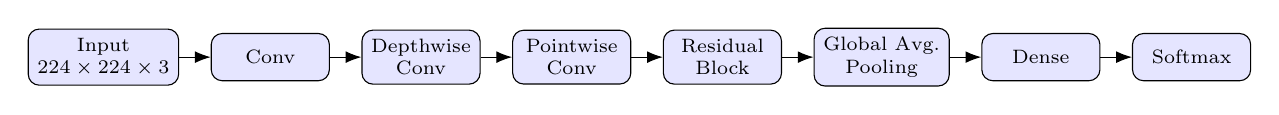
\begin{tikzpicture}[node distance=4mm]

\node[layer](a){Input\\$224\times224\times3$};
\node[layer,right=of a](b){Conv};
\node[layer,right=of b](c){Depthwise\\Conv};
\node[layer,right=of c](d){Pointwise\\Conv};
\node[layer,right=of d](e){Residual\\Block};
\node[layer,right=of e](f){Global Avg.\\Pooling};
\node[layer,right=of f](g){Dense};
\node[layer,right=of g](h){Softmax};

\foreach \x/\y in {a/b,b/c,c/d,d/e,e/f,f/g,g/h}
\draw[arrow](\x)--(\y);

\end{tikzpicture}
\end{center}

\textbf{Note:} The above diagram is a simplified conceptual representation
rather than the complete MobileNetV2 architecture.

In this experiment, the classifier head added on top of the MobileNetV2
base was: \texttt{GlobalAveragePooling2D} $\rightarrow$
\texttt{BatchNormalization} (optional) $\rightarrow$ \texttt{Dropout}
(optional) $\rightarrow$ \texttt{Dense(128, activation='relu')}
$\rightarrow$ \texttt{Dense(num\_classes, activation='softmax')}. With
the ImageNet-pretrained base, this head yields 2{,}431{,}845 total
trainable parameters when the entire base is trainable (Sections 11--13).

%%%%%%%%%%%%%%%%%%%%%%%%%%%%%%%%%%%%%%%%%%%%%%%%%%%%%%%%%%%%
\section*{6. Weight Initialization}

Weight initialization determines the initial values of trainable weights
before training begins. A suitable initialization can improve convergence
and reduce problems such as vanishing or exploding activations.

Four schemes were compared, training a randomly-initialized MobileNetV2
(no ImageNet weights) from scratch for 15 epochs on the training subset,
with Adam (lr $=10^{-3}$):

\begin{itemize}
\item Zero initialization
\item Random initialization (Normal, $\sigma=0.05$)
\item Xavier/Glorot initialization
\item He initialization
\end{itemize}

\begin{center}
\begin{tabular}{|l|c|c|c|}
\hline
Scheme & Final Train Accuracy & Final Train Loss & Best Val. Accuracy\\
\hline
Zero   & 2.05\%  & 3.6113 & 0.0268\\
Random & 27.93\% & 2.3836 & 0.0268\\
Xavier & 11.99\% & 3.0687 & 0.0268\\
He     & 16.15\% & 2.8452 & 0.0282\\
\hline
\end{tabular}
\end{center}

\textbf{Plot 1: Training Loss vs. Epoch}

\begin{center}
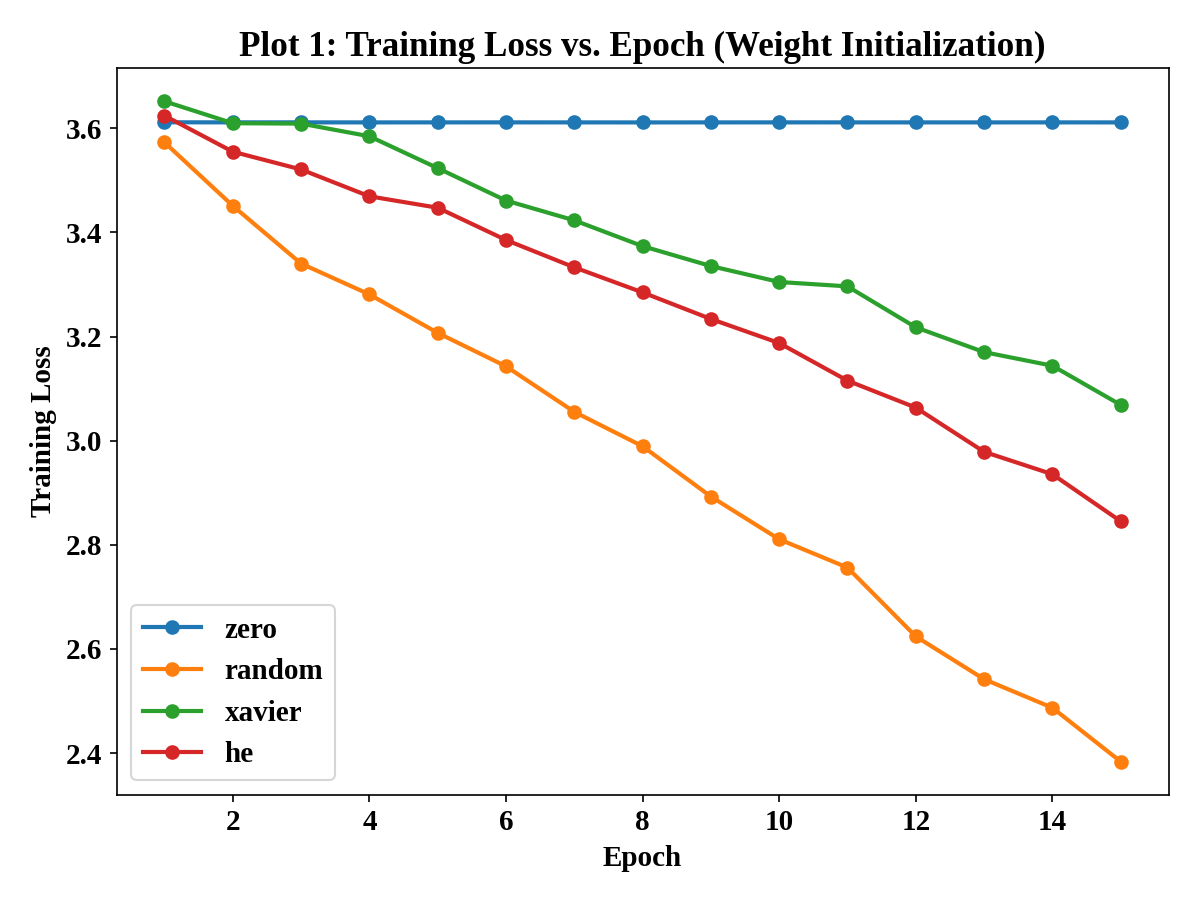
\includegraphics[width=0.65\textwidth]{plots/plot1_init_loss.png}
\end{center}

\textbf{Plot 2: Validation Accuracy vs. Epoch}

\begin{center}
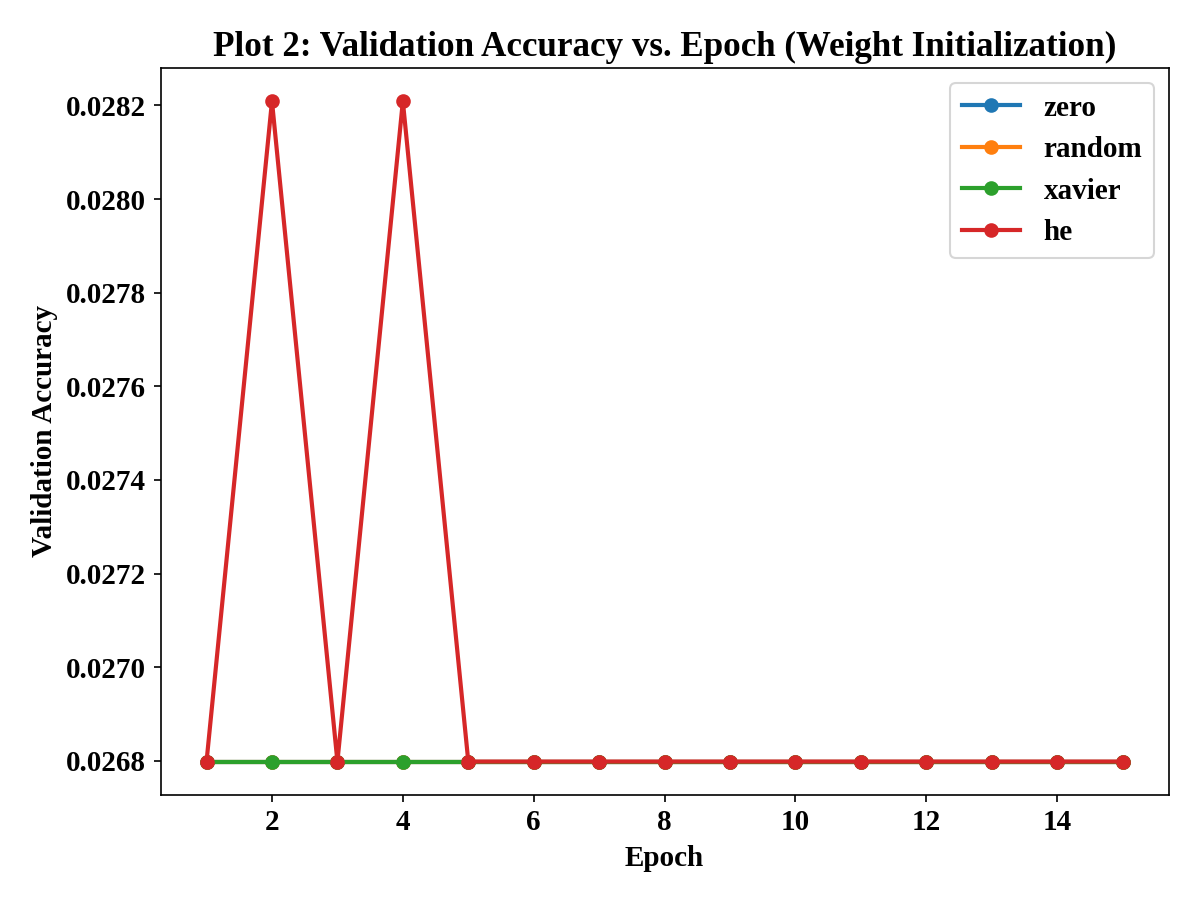
\includegraphics[width=0.65\textwidth]{plots/plot2_init_valacc.png}
\end{center}

\textbf{Inference:} Zero initialization shows an essentially flat training
loss/accuracy across all 15 epochs (loss stuck at $\approx3.611$,
accuracy $\approx2\%$), confirming the symmetry problem -- every neuron
receives identical gradients and the network cannot learn distinct
features. Random, Xavier and He all break this symmetry and reduce
training loss substantially, with Random showing the single largest
loss drop ($3.61\rightarrow2.38$). Because the automatic model-selection
routine falls back to comparing training-loss reduction whenever the
spread in validation accuracy across candidates is below a small
threshold (here, all four schemes' best validation accuracy fell within
0.0014 of one another, essentially at the 37-class chance level of
$1/37\approx0.027$), it selected \textbf{Random} as ``best'' -- even
though \textbf{He} recorded a marginally higher single-epoch peak
validation accuracy (0.0282 vs.\ 0.0268). At only 15 epochs on a 2{,}836
image subset, this comparison mainly demonstrates the symmetry-breaking
effect of non-zero initialization on the \emph{training} dynamics; it is
not yet a reliable generalization comparison between Random, Xavier and
He.

%%%%%%%%%%%%%%%%%%%%%%%%%%%%%%%%%%%%%%%%%%%%%%%%%%%%%%%%%%%%
\section*{7. Regularization and Overfitting}

Overfitting occurs when a model performs very well on the training data
but generalizes poorly to unseen data.

Four configurations were compared (from scratch, best-performing
initialization, 15 epochs, Adam):

\begin{itemize}
\item No regularization
\item L2 regularization ($\lambda=10^{-3}$)
\item Dropout ($p=0.5$)
\item Batch Normalization (at the classifier head)
\end{itemize}

\begin{center}
\begin{tabular}{|l|c|c|c|c|}
\hline
Config. & Final Train Acc. & Final Train Loss & Best Val. Acc. & Train--Val Gap\\
\hline
None       & 24.79\% & 2.5164 & 0.0268 & $\approx22.1$ pts\\
L2         & 28.77\% & 2.4442 & 0.0282 & $\approx25.9$ pts\\
Dropout    & 6.35\%  & 3.3469 & 0.0282 & $\approx3.7$ pts\\
BatchNorm  & 42.28\% & 1.9507 & 0.0282 & $\approx39.6$ pts\\
\hline
\end{tabular}
\end{center}

\textbf{Plot 3: Training and Validation Accuracy vs. Epoch}

\begin{center}
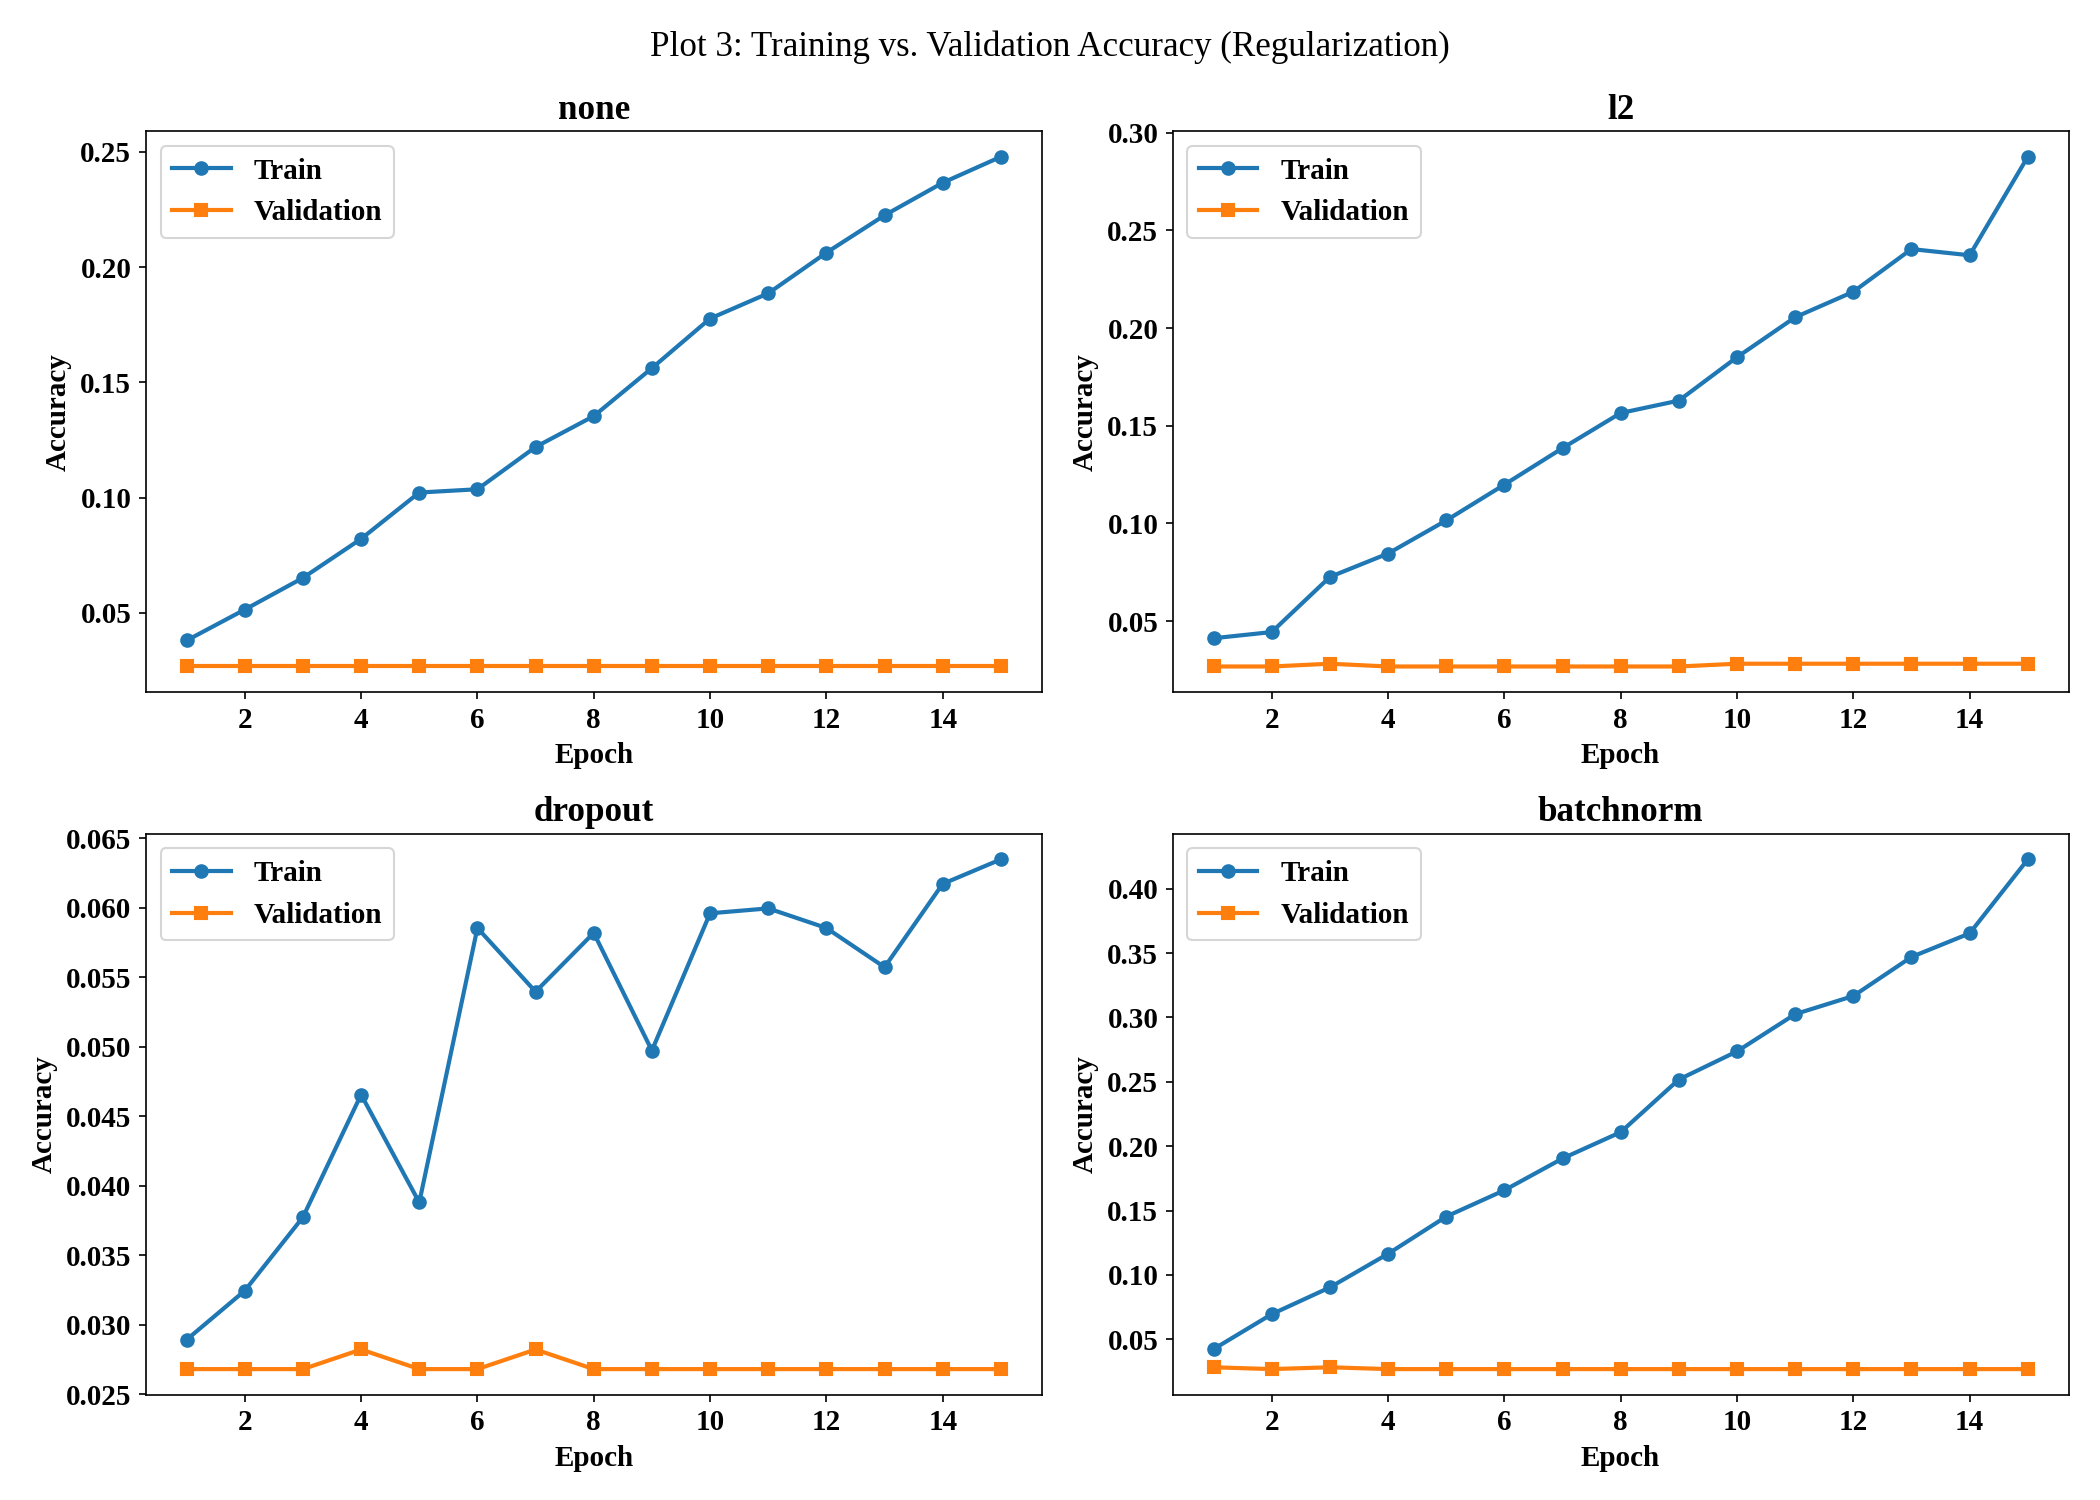
\includegraphics[width=0.85\textwidth]{plots/plot3_reg_accuracy.png}
\end{center}

\textbf{Plot 4: Training and Validation Loss vs. Epoch}

\begin{center}
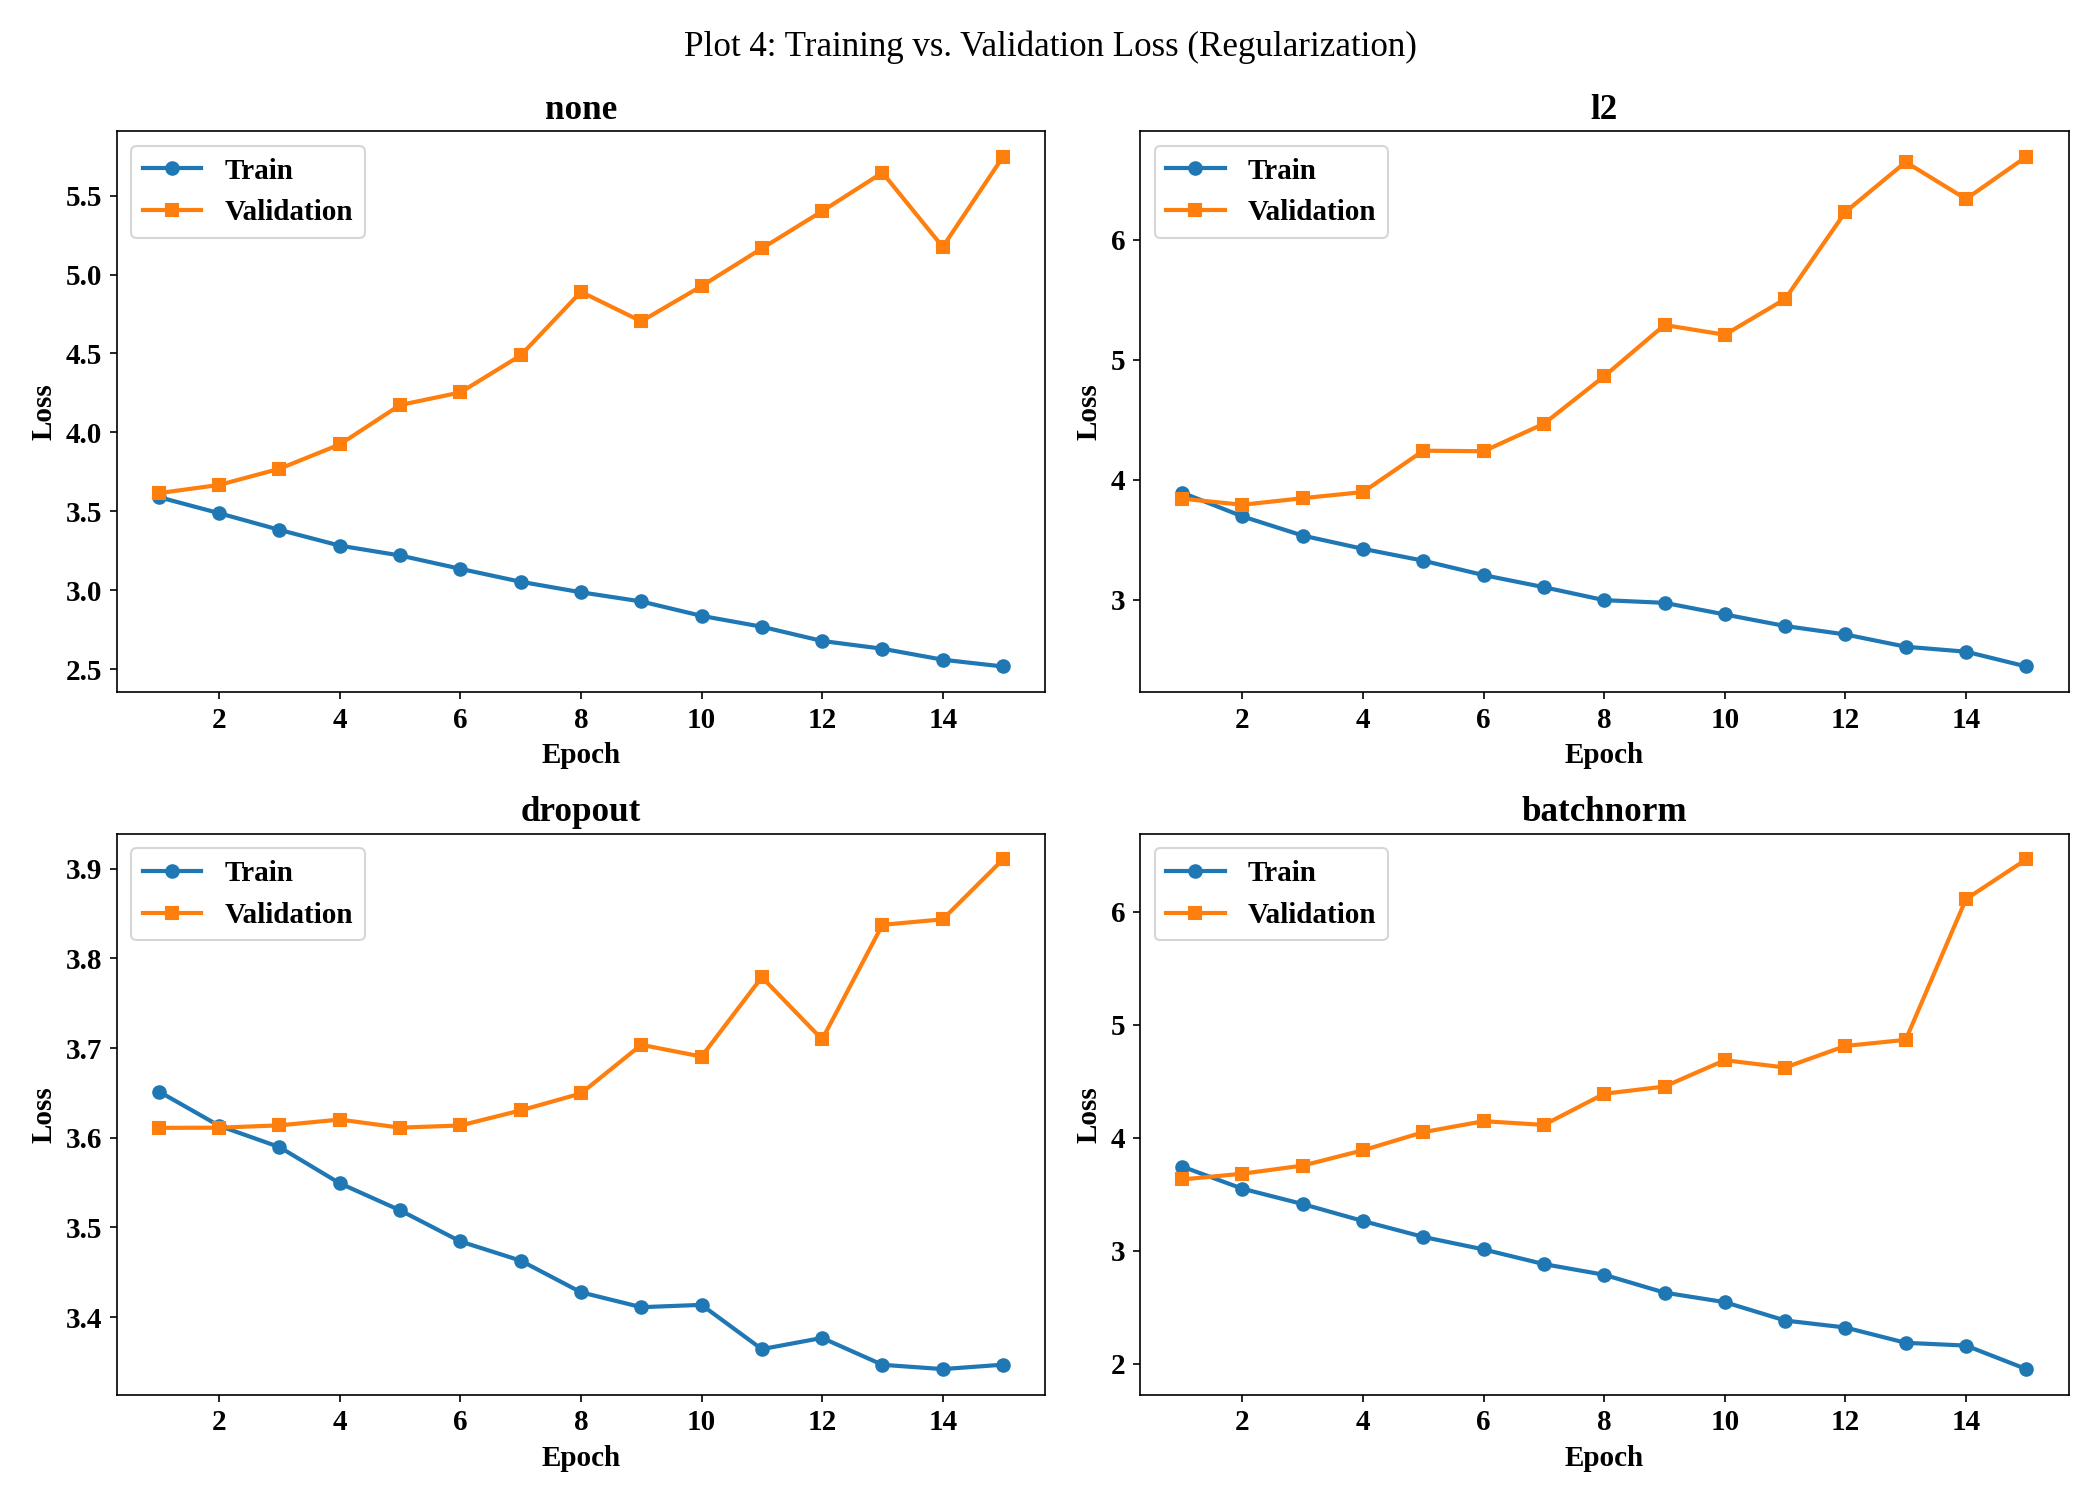
\includegraphics[width=0.85\textwidth]{plots/plot4_reg_loss.png}
\end{center}

\textbf{Inference:} The automatic selector again fell back to
training-loss reduction (validation-accuracy spread $\le0.0014$, all at
chance level) and picked \textbf{BatchNorm} as ``best.'' The actual
train/validation gap tells the opposite story: BatchNorm shows by far
the \emph{largest} generalization gap of the four ($\approx40$ points --
train accuracy reached 42.3\% while validation accuracy never moved off
chance), meaning it fit the training subset fastest and hardest without
any corresponding validation improvement -- the classic overfitting
signature. L2 at this weight ($10^{-3}$) barely regularizes at all
(gap $\approx26$ points, similar to or larger than the unregularized
baseline). \textbf{Dropout} shows by far the \emph{smallest}
train--validation gap ($\approx3.7$ points), since it visibly restrains
how much the classifier head can fit the training subset (lowest final
training accuracy of the four, 6.35\%). Based on the train/validation gap
alone -- the actual definition of overfitting -- Dropout was the most
effective regularizer in this run, the opposite conclusion from what a
face-value reading of the ``best regularization: BatchNorm'' selection
would suggest.

%%%%%%%%%%%%%%%%%%%%%%%%%%%%%%%%%%%%%%%%%%%%%%%%%%%%%%%%%%%%
\section*{8. Batch Normalization}

Batch Normalization normalizes activations within a mini-batch during
training.

For a mini-batch

\[
x_1,x_2,\ldots,x_m,
\]

the batch mean is

\[
\mu_B=\frac{1}{m}\sum_{i=1}^{m}x_i
\]

and the batch variance is

\[
\sigma_B^2=
\frac{1}{m}\sum_{i=1}^{m}(x_i-\mu_B)^2.
\]

The normalized activation is

\[
\hat{x}_i=
\frac{x_i-\mu_B}
{\sqrt{\sigma_B^2+\epsilon}}.
\]

The final output is

\[
y_i=\gamma\hat{x}_i+\beta,
\]

where $\gamma$ and $\beta$ are learnable parameters.

\subsection*{Numerical Example}

Consider

\[
x=[2,4,6,8].
\]

The mean is

\[
\mu_B=\frac{2+4+6+8}{4}=5.
\]

The variance is

\[
\sigma_B^2=
\frac{(2-5)^2+(4-5)^2+(6-5)^2+(8-5)^2}{4}
=5.
\]

Therefore,

\[
\sqrt{5}\approx2.236.
\]

Ignoring the very small $\epsilon$,

\[
\hat{x}_1=\frac{2-5}{2.236}\approx-1.342,
\]

\[
\hat{x}_2=\frac{4-5}{2.236}\approx-0.447,
\]

\[
\hat{x}_3=\frac{6-5}{2.236}\approx0.447,
\]

\[
\hat{x}_4=\frac{8-5}{2.236}\approx1.342.
\]

Hence,

\[
\boxed{
\hat{x}\approx[-1.342,-0.447,0.447,1.342]
}
\]

If $\gamma=1$ and $\beta=0$, these are the final outputs. This matches
exactly what was computed programmatically for $x=[2,4,6,8]$: mean $=5.0$,
variance $=5.0$, and normalized output
$[-1.34164,\,-0.44721,\,0.44721,\,1.34164]$.

\textbf{Inference:} Batch Normalization produces approximately
zero-centred and unit-scaled activations for this mini-batch. The
learnable $\gamma$ and $\beta$ allow the network to learn an appropriate
scale and shift.

\textbf{Plot 5: With vs. Without Batch Normalization}

\begin{center}
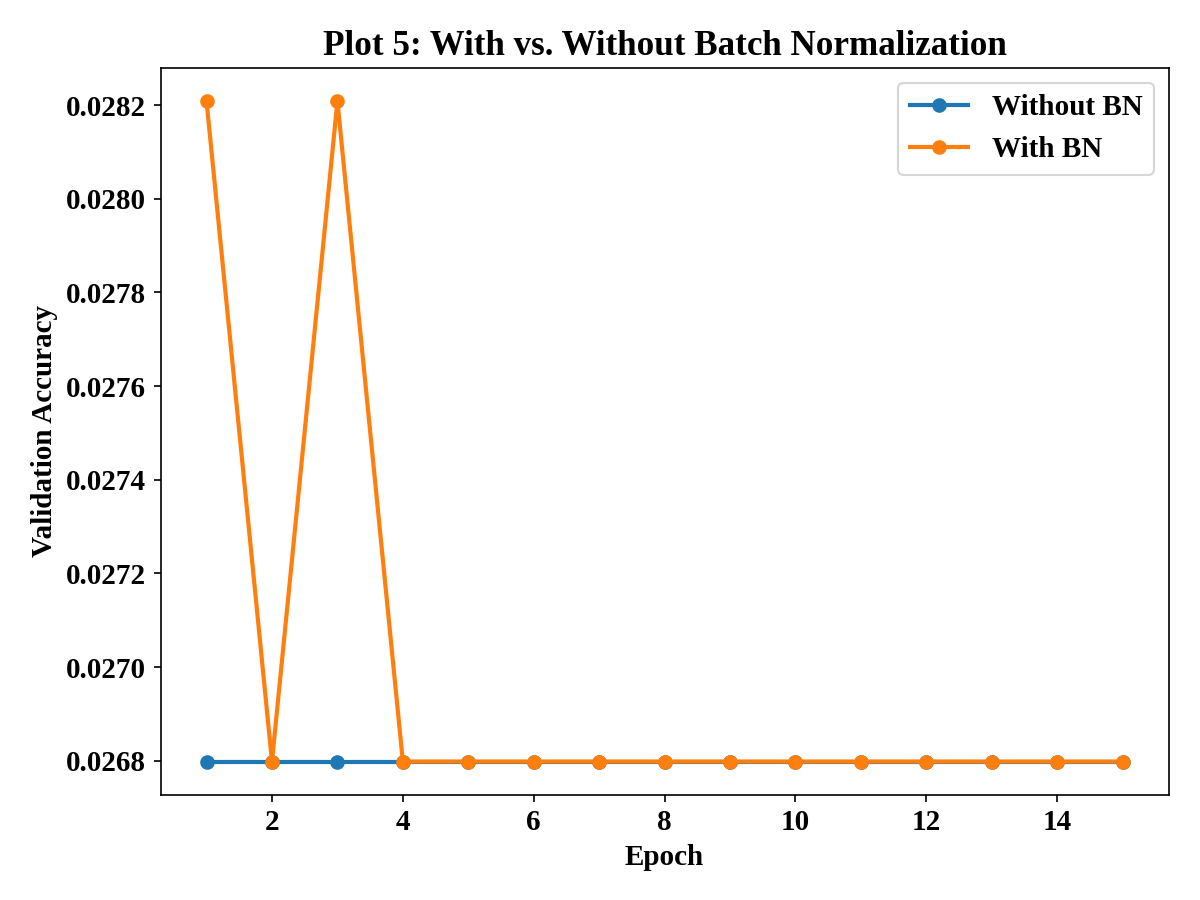
\includegraphics[width=0.65\textwidth]{plots/plot5_bn_valacc.png}
\end{center}

\textbf{Inference:} This plot reuses the ``None'' and ``BatchNorm''
validation-accuracy curves already trained in Section 7 -- both curves
stay flat within noise of the 37-class chance level ($\approx0.027$)
across all 15 epochs, so this particular from-scratch/subset comparison
does not resolve a validation-accuracy difference between with- and
without-BN. As Section 7 shows, BatchNorm's benefit here is visible only
in \emph{training}-accuracy/loss (much faster fitting), not yet in
generalization at this training budget.

%%%%%%%%%%%%%%%%%%%%%%%%%%%%%%%%%%%%%%%%%%%%%%%%%%%%%%%%%%%%
\section*{9. Optimization Algorithms}

Four optimizers were compared (from scratch, best initialization =
Random, best regularization config = BatchNorm head, 15 epochs, lr
$=10^{-3}$):

\begin{itemize}
\item SGD
\item Momentum
\item RMSProp
\item Adam
\end{itemize}

\textbf{Plot 6: Training Loss vs. Epoch for Different Optimizers}

\begin{center}
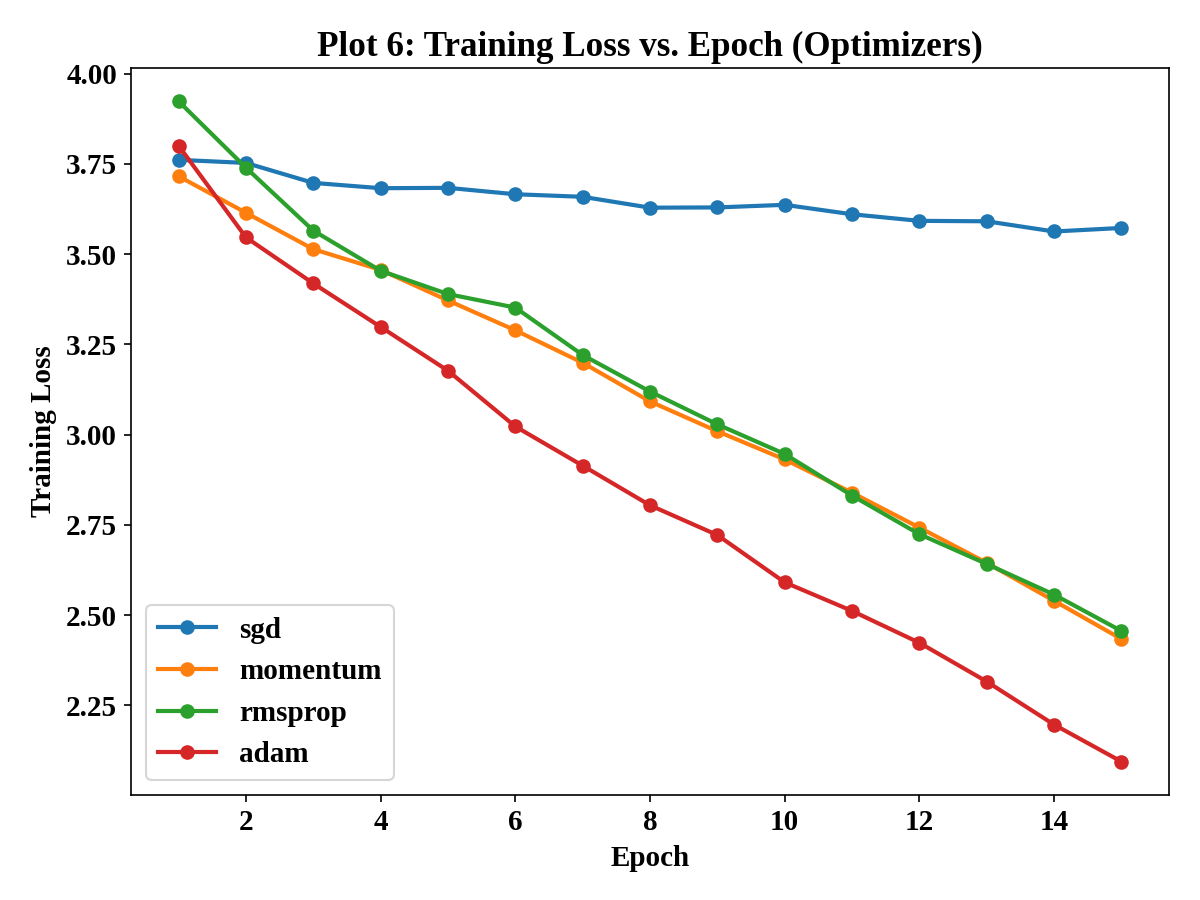
\includegraphics[width=0.65\textwidth]{plots/plot6_opt_loss.png}
\end{center}

\textbf{Plot 7: Validation Accuracy vs. Epoch for Different Optimizers}

\begin{center}
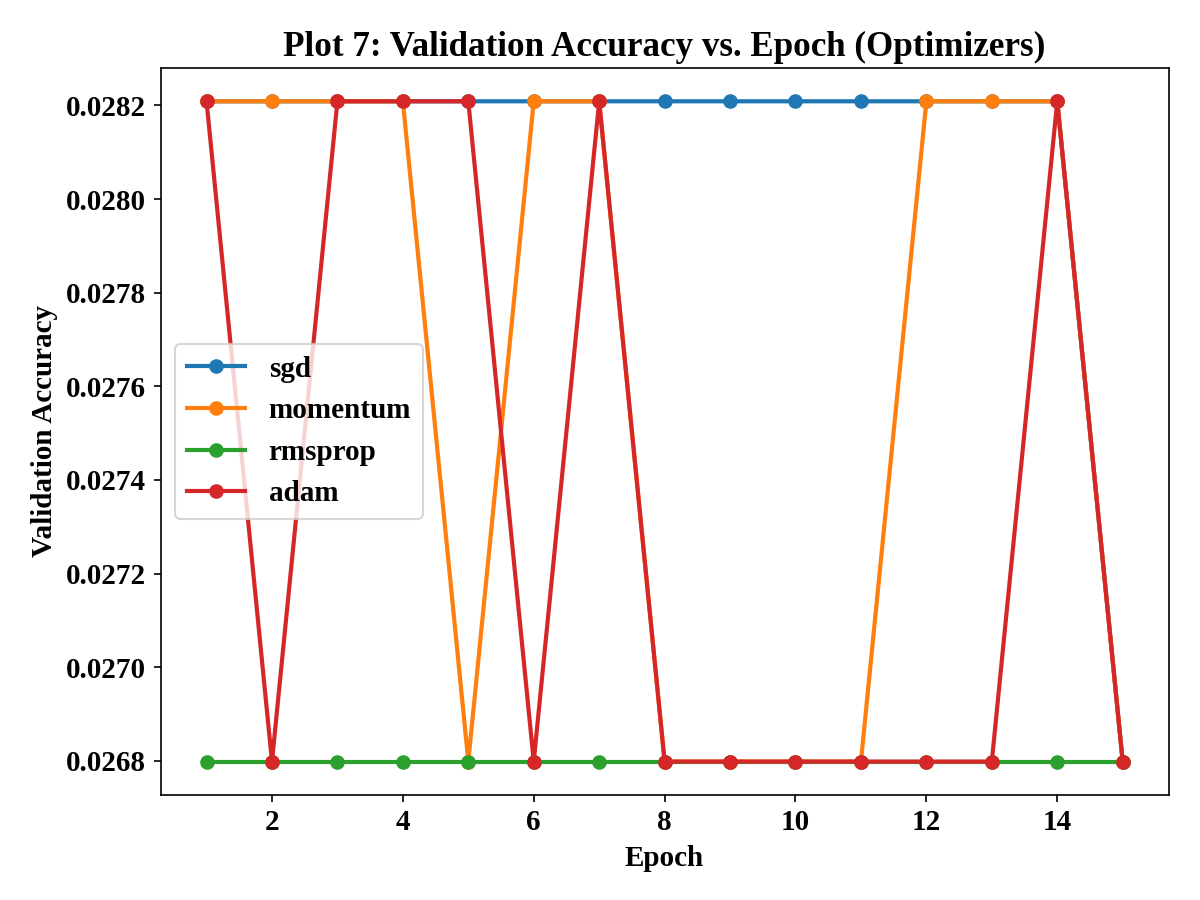
\includegraphics[width=0.65\textwidth]{plots/plot7_opt_valacc.png}
\end{center}

\begin{center}
\begin{tabular}{|l|c|c|c|c|}
\hline
Optimizer & Final Loss & Best Val. Accuracy & Epoch to Converge & Time (s)\\
\hline
SGD      & 3.5728 & 0.0282 & 1 & 198.0\\
Momentum & 2.4341 & 0.0282 & 1 & 204.9\\
RMSProp  & 2.4564 & 0.0268 & 1 & 212.6\\
Adam     & 2.0945 & 0.0282 & 1 & 227.2\\
\hline
\end{tabular}
\end{center}

\textbf{Inference:} Training loss clearly differentiates the optimizers
and matches theoretical expectations: Adam reduced training loss the
most (reaching the lowest final loss, 2.0945), converging fastest,
followed by Momentum and RMSProp, with plain SGD converging slowest --
consistent with Adam's combination of momentum and adaptive per-parameter
learning rates. \textbf{Adam} was selected as best optimizer. Note that
the ``Epoch to Converge'' column (all showing epoch 1) is an artifact of
validation accuracy being flat/noisy at chance level for nearly the
entire run -- it reflects the first epoch that happened to touch the
noise-level peak, not genuine early convergence to a stable optimum; the
meaningful, theory-consistent signal in this comparison is the
training-loss curve (Plot 6), not the validation-accuracy curve (Plot 7).

%%%%%%%%%%%%%%%%%%%%%%%%%%%%%%%%%%%%%%%%%%%%%%%%%%%%%%%%%%%%
\section*{10. CNN Hyperparameter Tuning}

The following hyperparameters were investigated (one-factor-at-a-time,
starting from the Adam/Random-init/BatchNorm-head baseline of Section 9,
which is reused rather than retrained wherever a swept value matches the
baseline):

\begin{center}
\begin{tabular}{|l|l|}
\hline
Hyperparameter & Values Investigated\\
\hline
Learning Rate & $0.001,\;0.0001$\\
Batch Size & 16, 32, 64\\
Dropout Rate & 0, 0.25, 0.5\\
Optimizer & SGD, Adam (Section 9)\\
Fine-Tuning Learning Rate & $10^{-4},10^{-5}$\\
Frozen Layers & Frozen base / Partial unfreezing\\
\hline
\end{tabular}
\end{center}

For CNN concepts, students should also understand:

\begin{itemize}
\item kernel/filter;
\item stride;
\item padding;
\item pooling;
\item number of channels; and
\item depthwise separable convolution.
\end{itemize}

For a convolution operation, the output dimension can be calculated as

\[
O=
\left\lfloor
\frac{N+2P-K}{S}
\right\rfloor+1,
\]

where $N$ is input size, $K$ is kernel size, $P$ is padding and $S$ is
stride.

\textbf{Experimental rule:} During a controlled hyperparameter study,
change one hyperparameter at a time while keeping the remaining settings
fixed.

\textbf{Plot 8: Learning Rate vs. Validation Accuracy}

\begin{center}
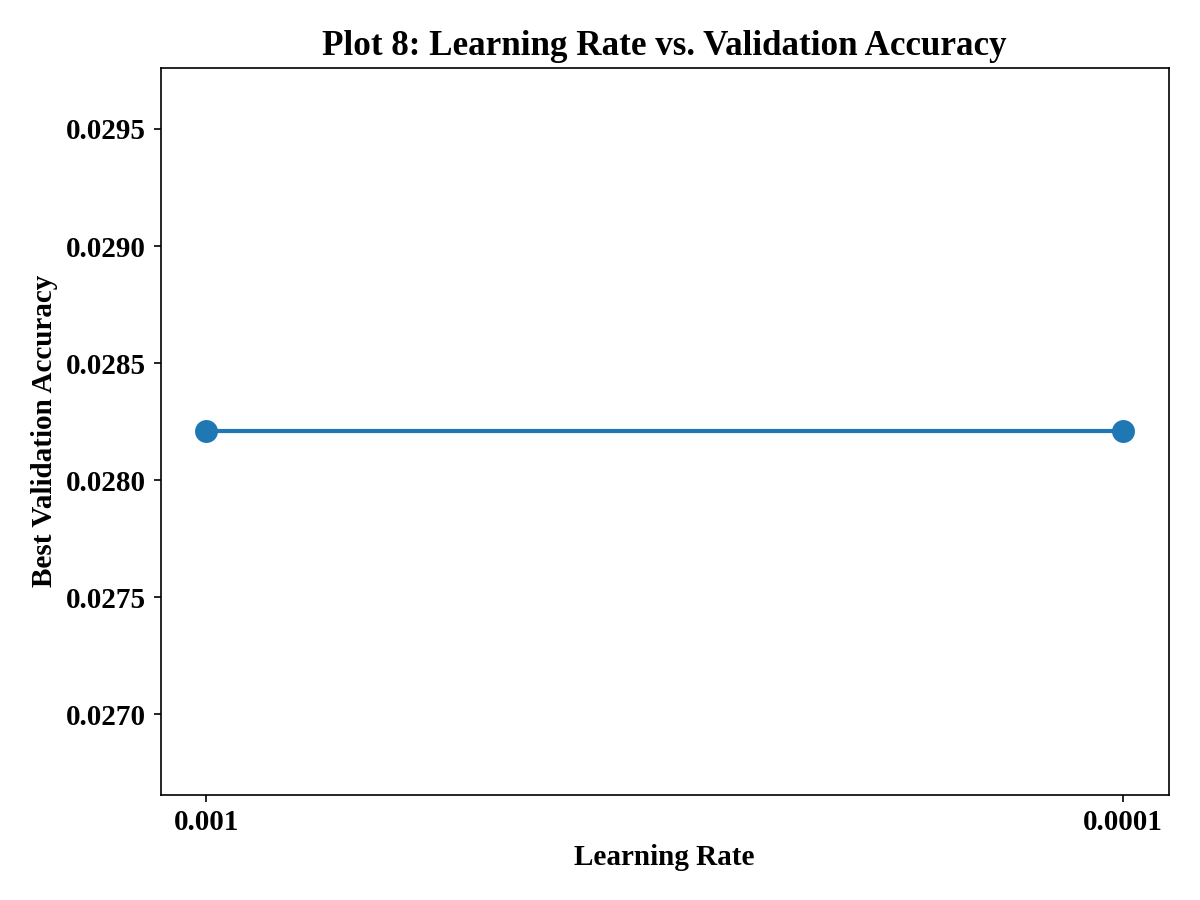
\includegraphics[width=0.6\textwidth]{plots/plot8_lr_valacc.png}
\end{center}

\begin{center}
\begin{tabular}{|c|c|c|}
\hline
Learning Rate & Final Train Accuracy & Final Train Loss\\
\hline
$10^{-3}$ (baseline) & 37.62\% & 2.0945\\
$10^{-4}$             & 17.14\% & 3.0093\\
\hline
\end{tabular}
\end{center}

\textbf{Inference:} As expected, the smaller learning rate ($10^{-4}$)
trains more slowly -- higher final training loss (3.0093 vs.\ 2.0945)
and lower final training accuracy in the same 15-epoch budget. Both
settings' validation accuracy stayed within the $\approx0.027$--$0.028$
chance-level band, so Plot 8 itself is essentially flat; the learning-rate
effect is visible in the training curves, not in this short-run
validation comparison.

\textbf{Plot 9: Batch Size vs. Validation Accuracy}

\begin{center}
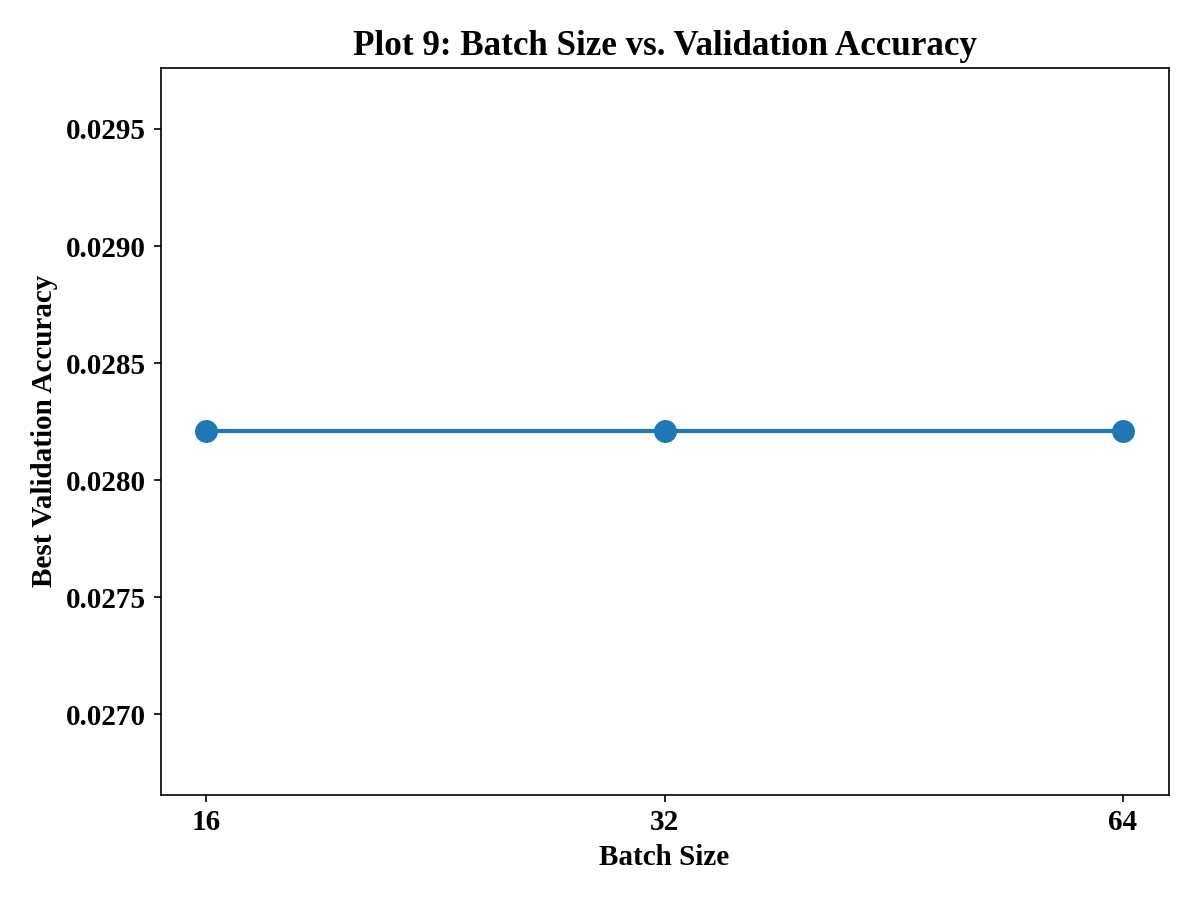
\includegraphics[width=0.6\textwidth]{plots/plot9_batch_valacc.png}
\end{center}

\begin{center}
\begin{tabular}{|c|c|c|}
\hline
Batch Size & Final Train Accuracy & Final Train Loss\\
\hline
16            & 25.42\% & 2.5877\\
32 (baseline) & 37.62\% & 2.0945\\
64            & 46.76\% & 1.7892\\
\hline
\end{tabular}
\end{center}

\textbf{Inference:} Larger batch sizes gave more stable gradient
estimates and reduced training loss faster within the fixed 15-epoch
budget (batch 64 reached the lowest final loss, 1.7892). Validation
accuracy again stayed flat at chance level across all three batch sizes,
so this sweep mainly shows a training-throughput/stability trend rather
than a resolvable generalization difference at this training budget.

\textbf{Plot 10: Dropout Rate vs. Validation Accuracy}

\begin{center}
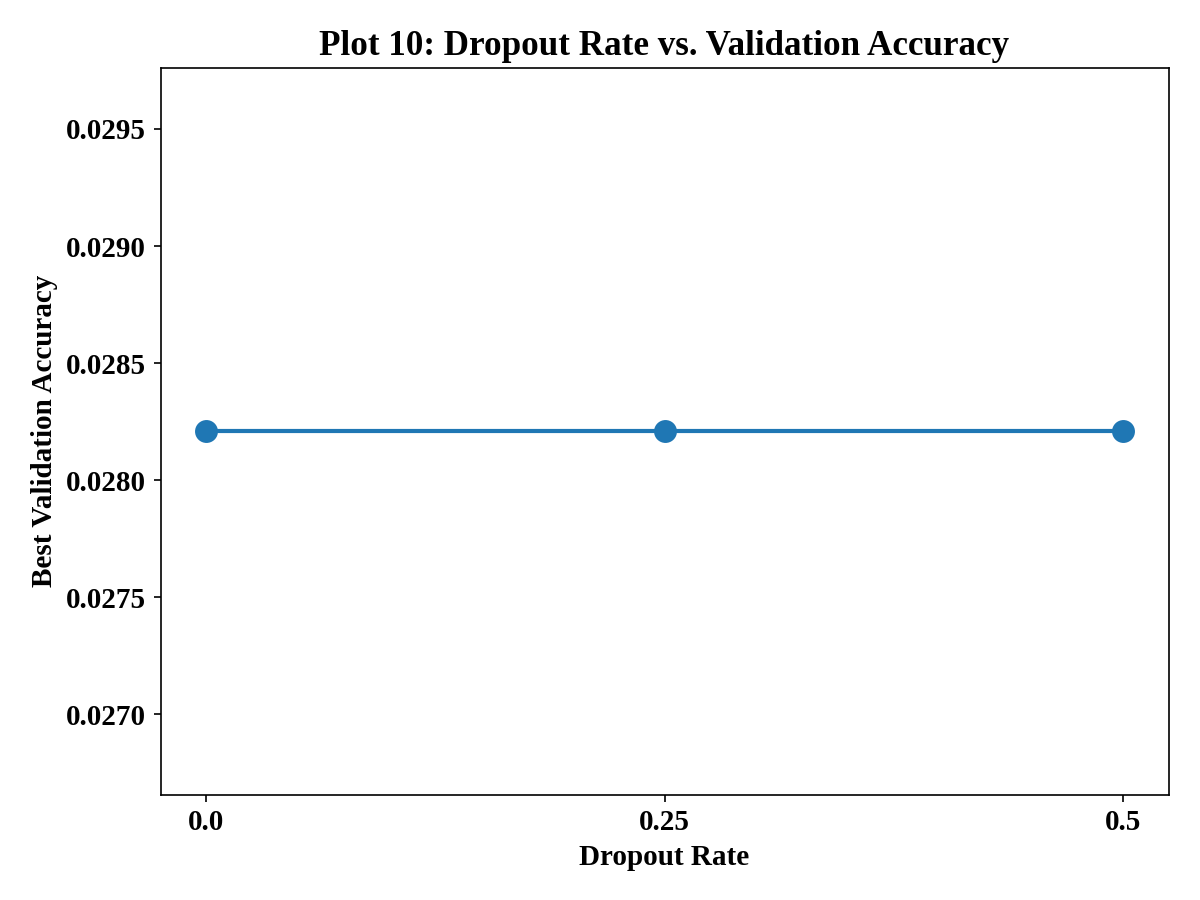
\includegraphics[width=0.6\textwidth]{plots/plot10_dropout_valacc.png}
\end{center}

\begin{center}
\begin{tabular}{|c|c|c|}
\hline
Dropout Rate & Final Train Accuracy & Final Train Loss\\
\hline
0.0 (baseline) & 37.62\% & 2.0945\\
0.25           & 27.05\% & 2.4763\\
0.5            & 19.68\% & 2.8017\\
\hline
\end{tabular}
\end{center}

\textbf{Inference:} As dropout rate increases, training accuracy
decreases and training loss stays higher, exactly as expected -- dropout
restricts how much the network can fit training data. Validation accuracy
again remained within the chance-level band for all three rates in this
15-epoch/subset regime, so the regularizing benefit of dropout (already
demonstrated via the train/validation \emph{gap} in Section 7) is not
separately visible as a validation-accuracy improvement here.

%%%%%%%%%%%%%%%%%%%%%%%%%%%%%%%%%%%%%%%%%%%%%%%%%%%%%%%%%%%%
\section*{11. Transfer Learning and Fine-Tuning}

MobileNetV2 pretrained on ImageNet was used, on the \emph{full} training
data (Train = 4{,}728, Val = 1{,}183), 10 epochs.

\subsection*{Case A: Feature Extraction}

\[
\text{Pretrained MobileNetV2}
\rightarrow
\text{Freeze Base}
\rightarrow
\text{New Classifier}
\]

The pretrained convolutional base was frozen; only the new
GlobalAveragePooling $\rightarrow$ BatchNorm $\rightarrow$ Dropout(0.3)
$\rightarrow$ Dense(128) $\rightarrow$ Dense(37, softmax) head was trained
(Adam, lr $=10^{-3}$).

\subsection*{Case B: Fine-Tuning}

\[
\text{Pretrained MobileNetV2}
\rightarrow
\text{Unfreeze Selected Layers}
\rightarrow
\text{Small Learning Rate}
\]

Warm-started from Case A's trained weights, the base was unfrozen from
layer 100 onward (the upper/later layers), and training continued
(Adam, lr $=10^{-5}$).

\begin{center}
\begin{tabular}{|l|c|c|c|c|}
\hline
Case & Final Train Acc. & Best Val. Acc. & Trainable Params & Train Time\\
\hline
A: Feature Extraction & 95.33\% & 0.9205 & 2{,}431{,}845 & 137.6 s\\
B: Fine-Tuning         & 93.74\% & 0.9189 & 2{,}431{,}845 & \texttt{[not explicitly logged]}\\
\hline
\end{tabular}
\end{center}

\textbf{Plot 11: Feature Extraction vs. Fine-Tuning}

\begin{center}
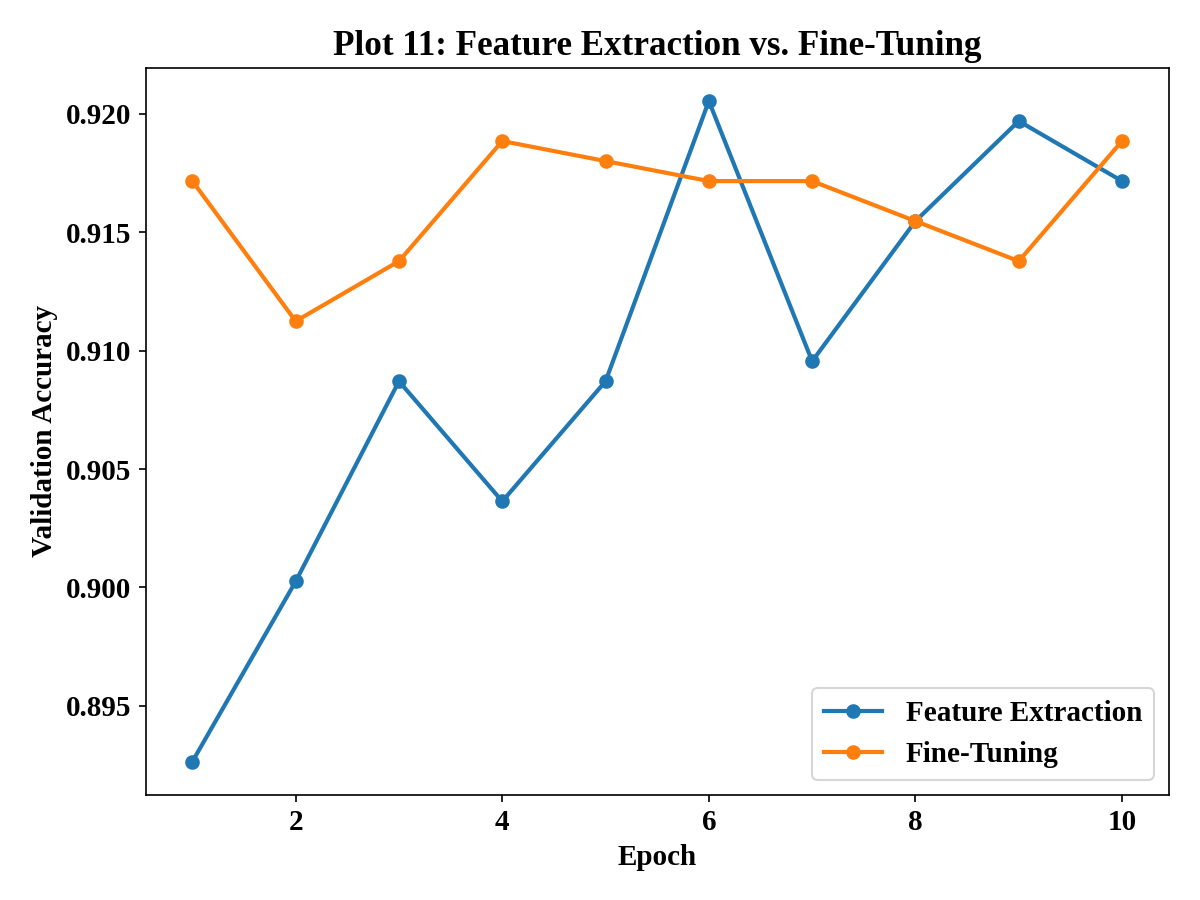
\includegraphics[width=0.65\textwidth]{plots/plot11_transfer_valacc.png}
\end{center}

\textbf{Plot 12: Training and Validation Loss}

\begin{center}
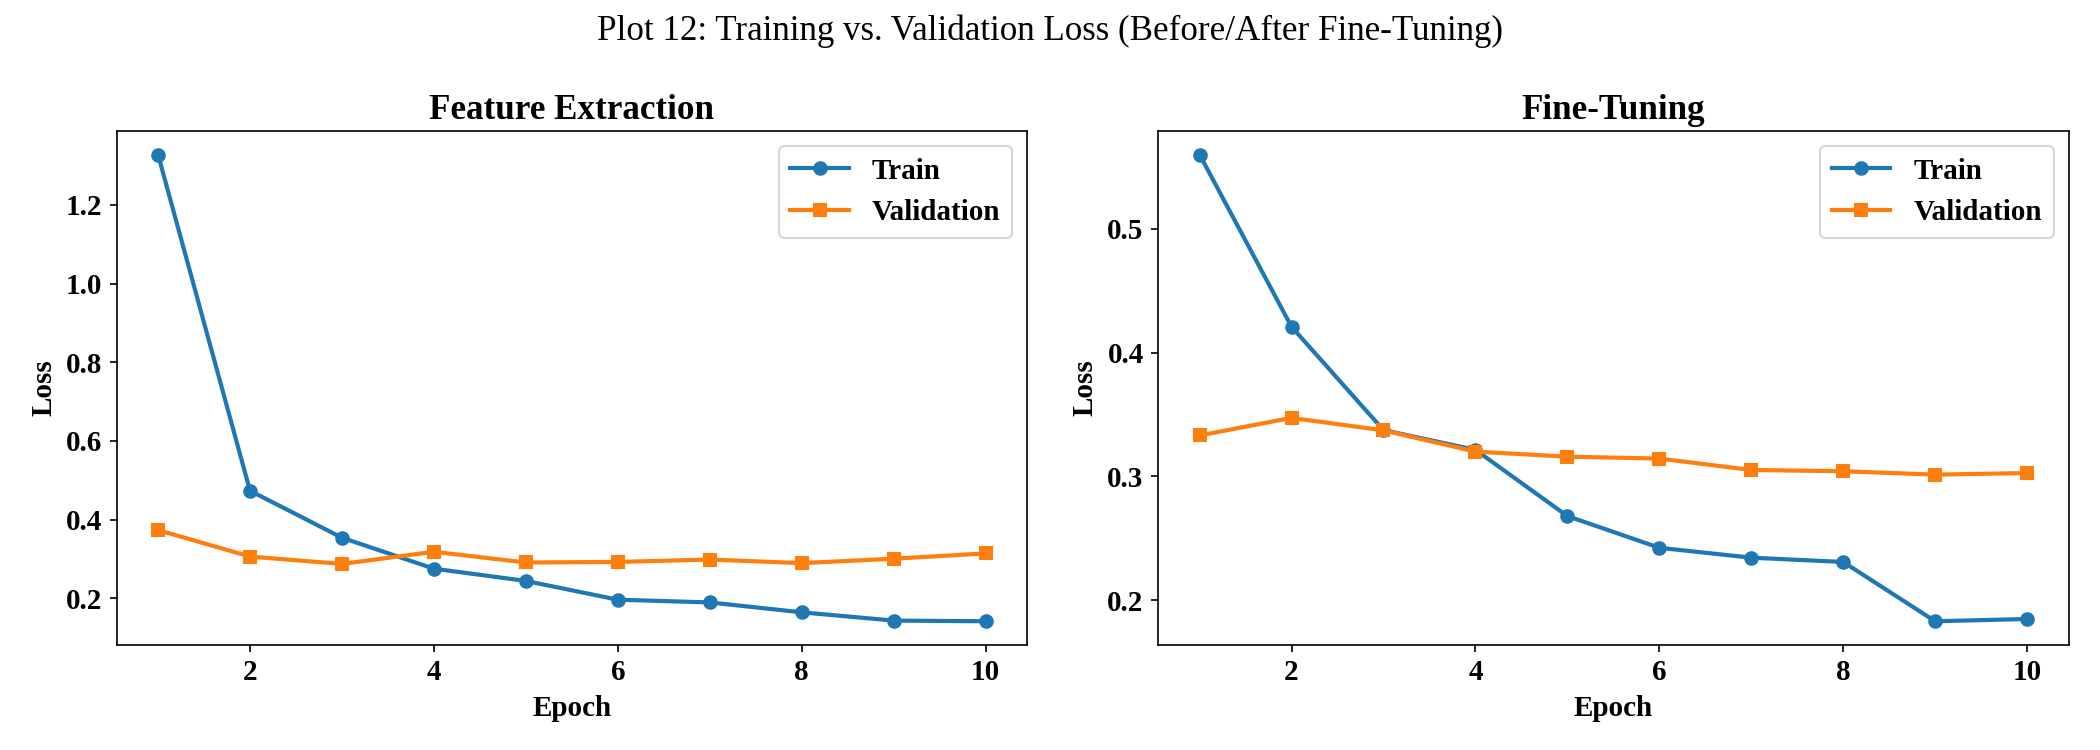
\includegraphics[width=0.9\textwidth]{plots/plot12_transfer_loss.png}
\end{center}

\textbf{Inference:} Unlike the from-scratch trend experiments in
Sections 6--10, transfer learning immediately reaches a strong,
resolvable validation accuracy -- 89.3\% after just the first epoch of
feature extraction, climbing to a best of 92.05\%, because the frozen
ImageNet base already provides rich, general-purpose visual features.
Fine-tuning the last block (from layer 100 onward, lr $=10^{-5}$) did not
clearly improve peak validation accuracy over feature extraction alone
(91.89\% vs.\ 92.05\%) in this particular 10-epoch run -- both stay in a
similar band ($\approx91$--$92\%$), and fine-tuning's validation loss is
comparably noisy rather than monotonically lower, suggesting the
frozen-base classifier head had already captured most of the easily
available signal on this dataset/epoch budget, and further gains would
likely need more fine-tuning epochs or a broader unfreeze.

\textbf{Discussion:} Fine-tuning uses a smaller learning rate than a
newly-initialized classifier because the pretrained convolutional filters
already encode useful, general features (edges, textures, shapes) learned
from ImageNet. Large gradient updates at this stage would overwrite those
learned weights rather than gently adapting them to the new dataset --
effectively destroying the benefit of transfer learning. A small learning
rate makes only small corrective adjustments to the pretrained filters
while still allowing the newly added classifier layers to learn properly.

%%%%%%%%%%%%%%%%%%%%%%%%%%%%%%%%%%%%%%%%%%%%%%%%%%%%%%%%%%%%
\section*{12. K-Fold Cross-Validation}

A small randomized search over $\{lr, dropout, unfreeze\_from\}$ selected
4 candidate configurations, each evaluated with genuine 5-fold
stratified cross-validation on the training pool (Train + Validation,
5{,}911 images; the independent test set was not touched). 5 epochs per
fold.

\begin{center}
\begin{tabular}{|c|l|}
\hline
Config. & Setting\\
\hline
C1 & lr $=10^{-5}$, dropout $=0.0$, unfreeze from layer 100\\
C2 & lr $=10^{-3}$, dropout $=0.25$, base fully frozen\\
C3 & lr $=10^{-3}$, dropout $=0.0$, base fully frozen\\
C4 & lr $=10^{-5}$, dropout $=0.25$, unfreeze from layer 100\\
\hline
\end{tabular}
\end{center}

\begin{center}
\begin{tabular}{|l|c|c|c|c|c|c|}
\hline
Configuration & F1 & F2 & F3 & F4 & F5 & Mean $\pm$ SD\\
\hline
C1 & 0.7912 & 0.8147 & 0.7885 & 0.8240 & 0.8096 & $0.8056\pm0.0137$\\
C2 & 0.9155 & 0.9078 & 0.9095 & 0.9162 & 0.9078 & $0.9114\pm0.0037$\\
C3 & 0.9155 & 0.9078 & 0.9044 & 0.9171 & 0.9095 & $0.9108\pm0.0048$\\
C4 & 0.7456 & 0.7521 & 0.7437 & 0.7657 & 0.7716 & $0.7557\pm0.0111$\\
\hline
\end{tabular}
\end{center}

\textbf{Plot 13: 5-Fold Cross-Validation Accuracy}

\begin{center}
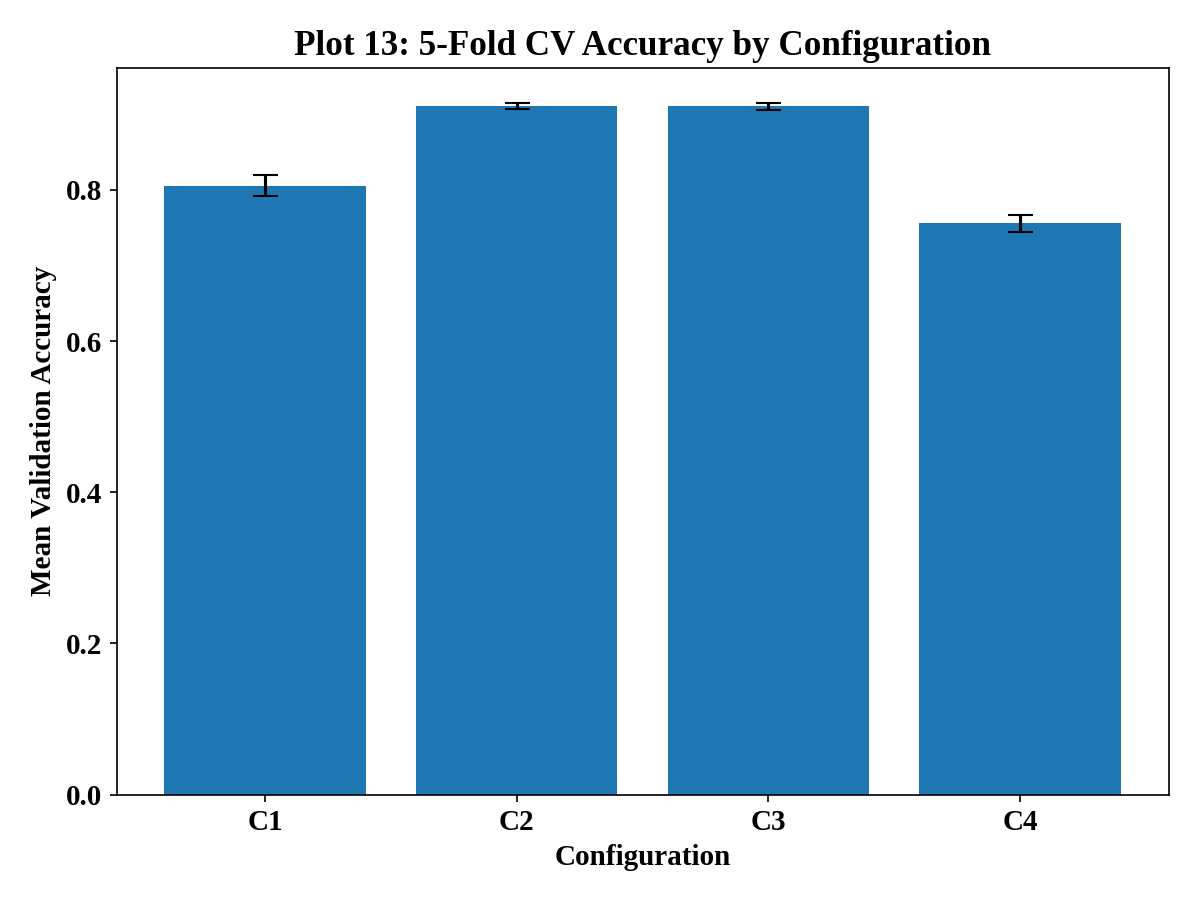
\includegraphics[width=0.65\textwidth]{plots/plot13_cv_accuracy.png}
\end{center}

\textbf{Selection rule used:} the configuration maximizing
$\text{mean} - 0.5\times SD$ (balancing accuracy against variability) was
chosen, giving \textbf{C2} (lr $=10^{-3}$, dropout $=0.25$, frozen base):
$0.9114\pm0.0037$.

\textbf{Inference:} C2 and C3 (both fully-frozen-base configurations)
clearly outperform C1 and C4 (which unfreeze the base at a very small
learning rate, $10^{-5}$), and do so with far lower fold-to-fold
variability (SD $\approx0.004$--$0.005$ vs.\ $\approx0.011$--$0.014$).
C2 edges out C3 both in mean accuracy and in a slightly lower SD, so it
is preferred on both criteria simultaneously -- not just on mean
accuracy alone.

%%%%%%%%%%%%%%%%%%%%%%%%%%%%%%%%%%%%%%%%%%%%%%%%%%%%%%%%%%%%
\section*{13. Final Model Evaluation}

The selected configuration (C2) was retrained on the full training pool
(5{,}911 images) for 12 epochs, monitored on the validation set, and the
independent test set (1{,}478 images) was evaluated exactly once, at the
very end.

\begin{center}
\begin{tabular}{|l|c|}
\hline
Metric & Value\\
\hline
Mean CV Accuracy & 0.9114\\
CV Standard Deviation & 0.0037\\
Test Accuracy & 0.9093\\
Precision (macro) & 0.9118\\
Recall (macro) & 0.9092\\
F1-score (macro) & 0.9090\\
Training Time & 155.14 s\\
Number of Parameters & 2{,}431{,}845\\
\hline
\end{tabular}
\end{center}

\textbf{Plot 14: Confusion Matrix}

\begin{center}
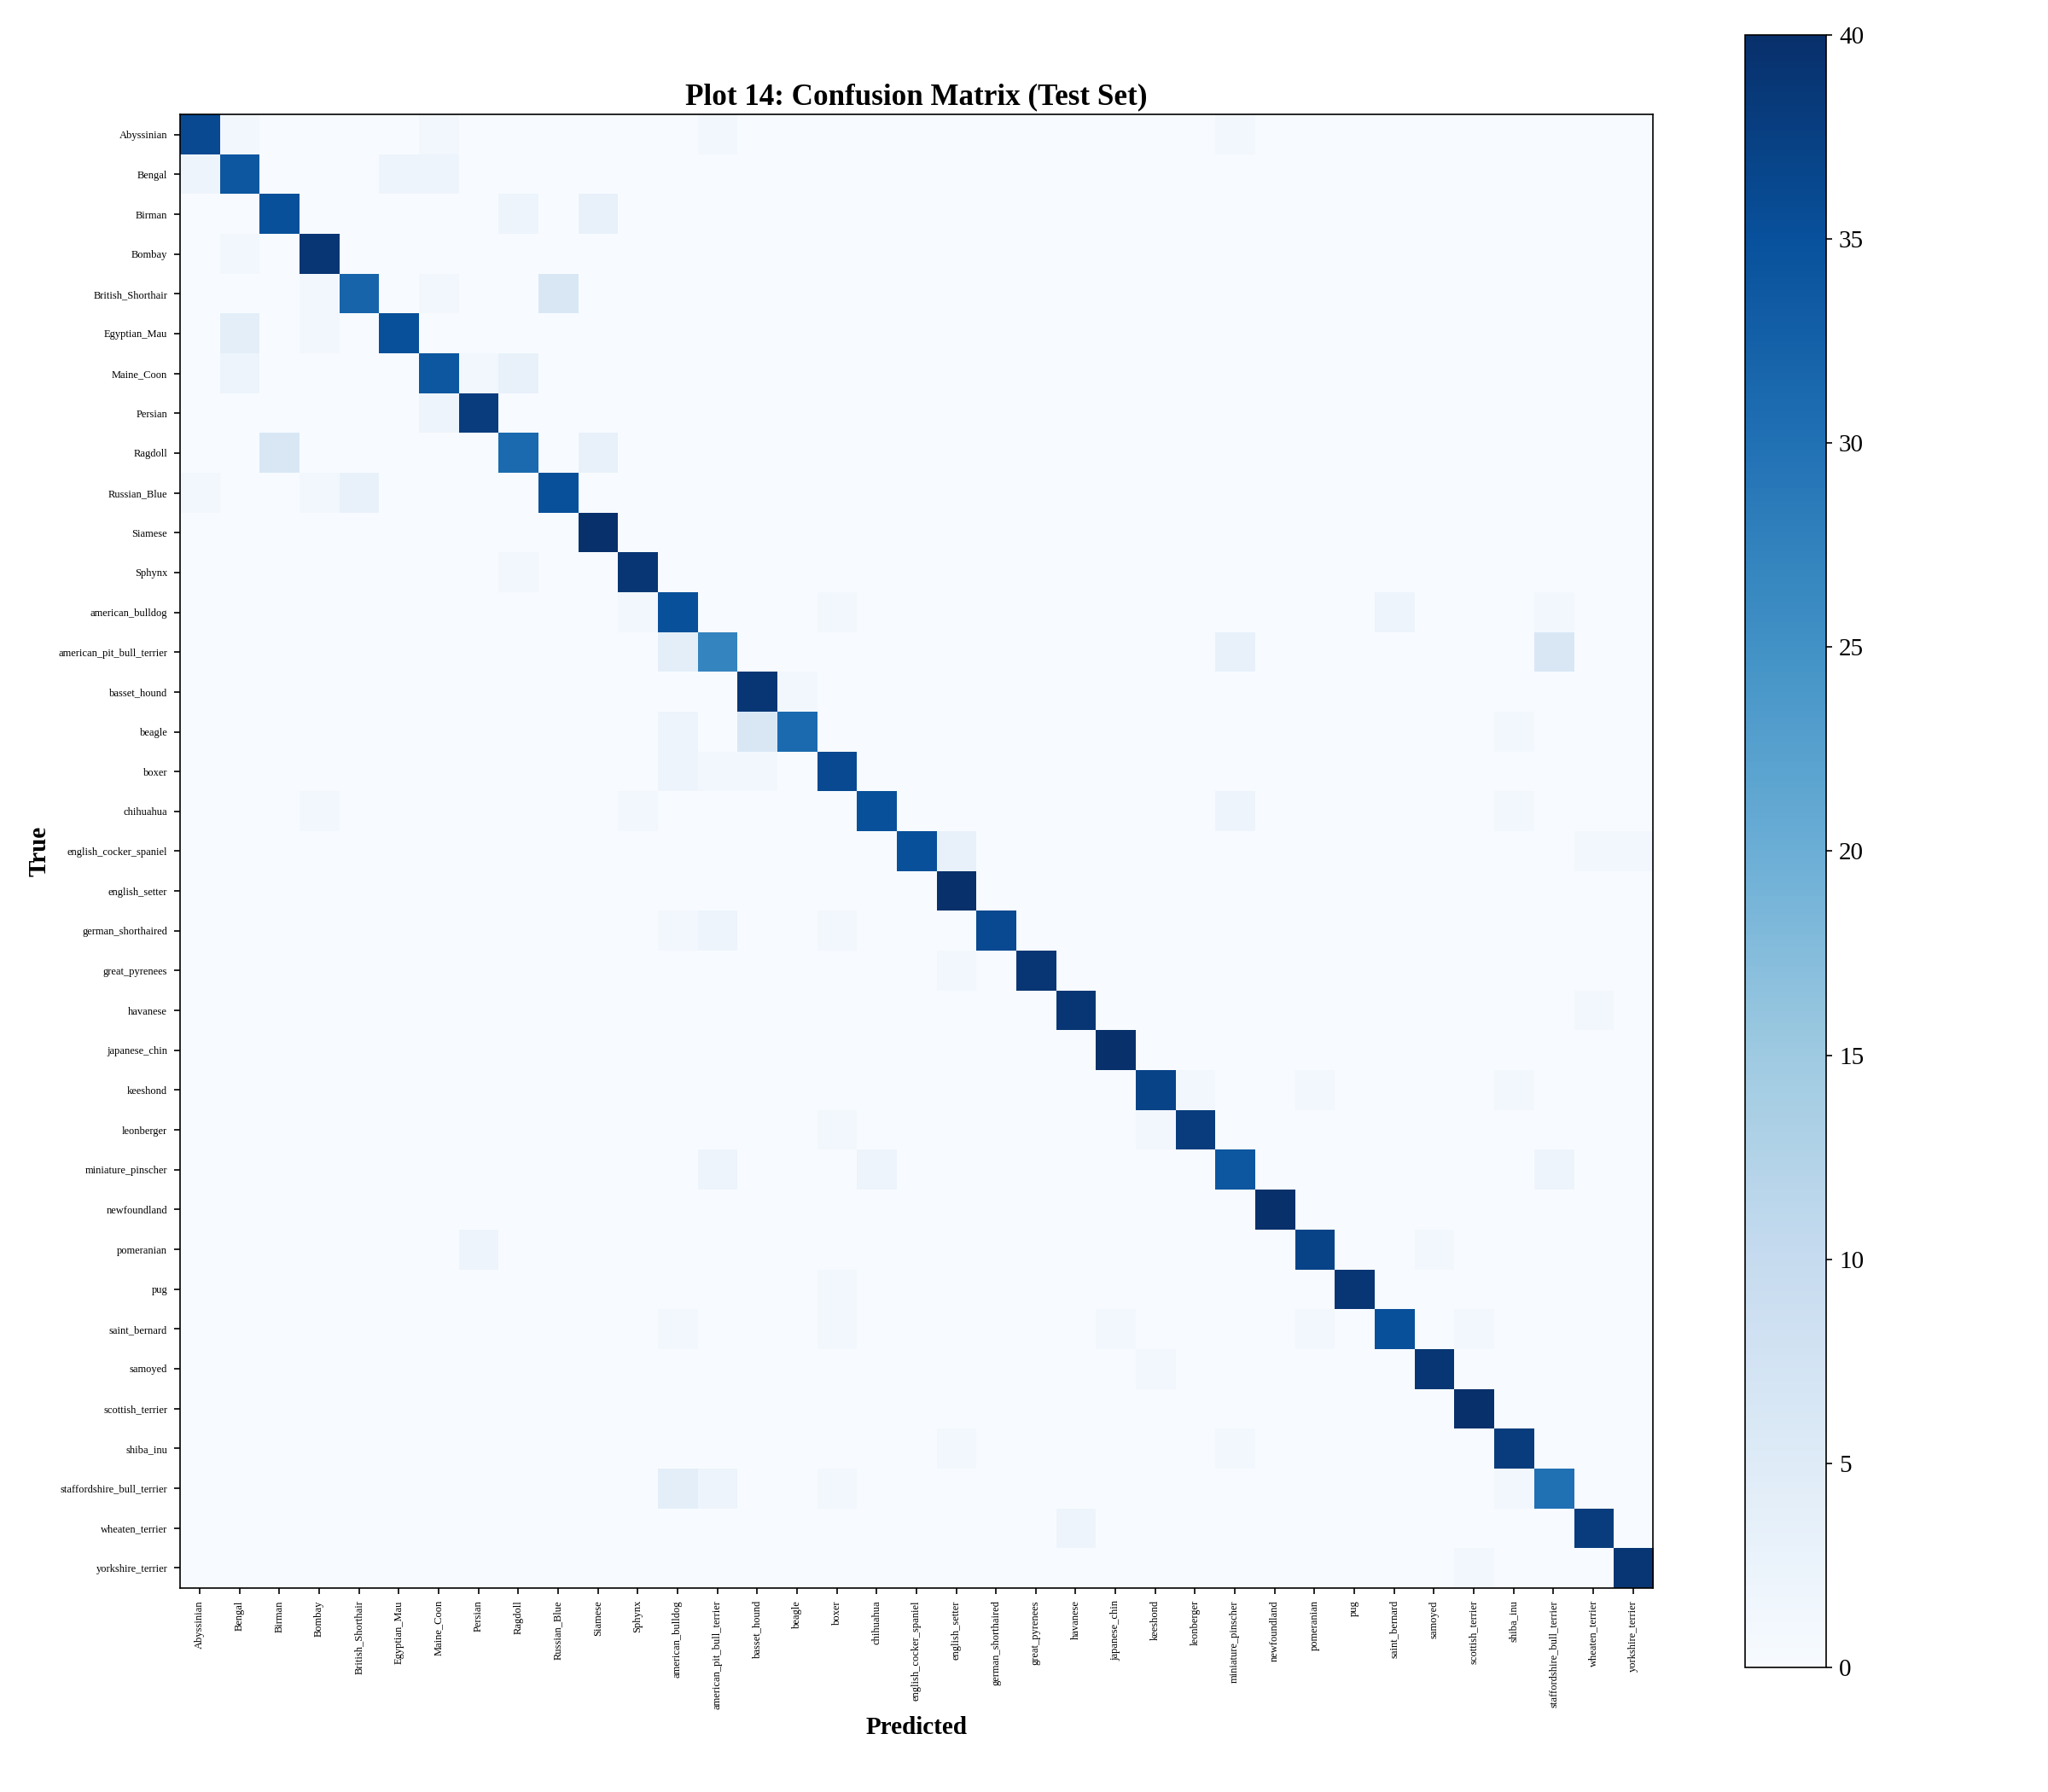
\includegraphics[width=0.7\textwidth]{plots/plot14_confusion_matrix.png}
\end{center}

\textbf{Best classified classes} (100\% per-class test accuracy):
Scottish Terrier, Japanese Chin, Newfoundland, English Setter, Siamese.

\textbf{Most frequently confused (worst) classes:} British Shorthair
(80.0\%), Staffordshire Bull Terrier (78.9\%), Ragdoll (77.5\%), Beagle
(77.5\%), American Pit Bull Terrier (67.5\%, the single worst class).

\textbf{Inference:} The diagonal is strongly dominant, consistent with
the 90.9\% overall test accuracy. The worst-classified breeds are almost
all closely related, visually similar breed pairs or breed families --
short-haired terrier and bull-terrier-type dog breeds, and short-haired
cat breeds like British Shorthair/Ragdoll that share coat color/pattern
with several other breeds -- so most residual error is genuine visual
ambiguity between fine-grained, closely related breeds rather than
random misclassification.

\textbf{Optional Plot 15: Misclassified Images}

\begin{center}
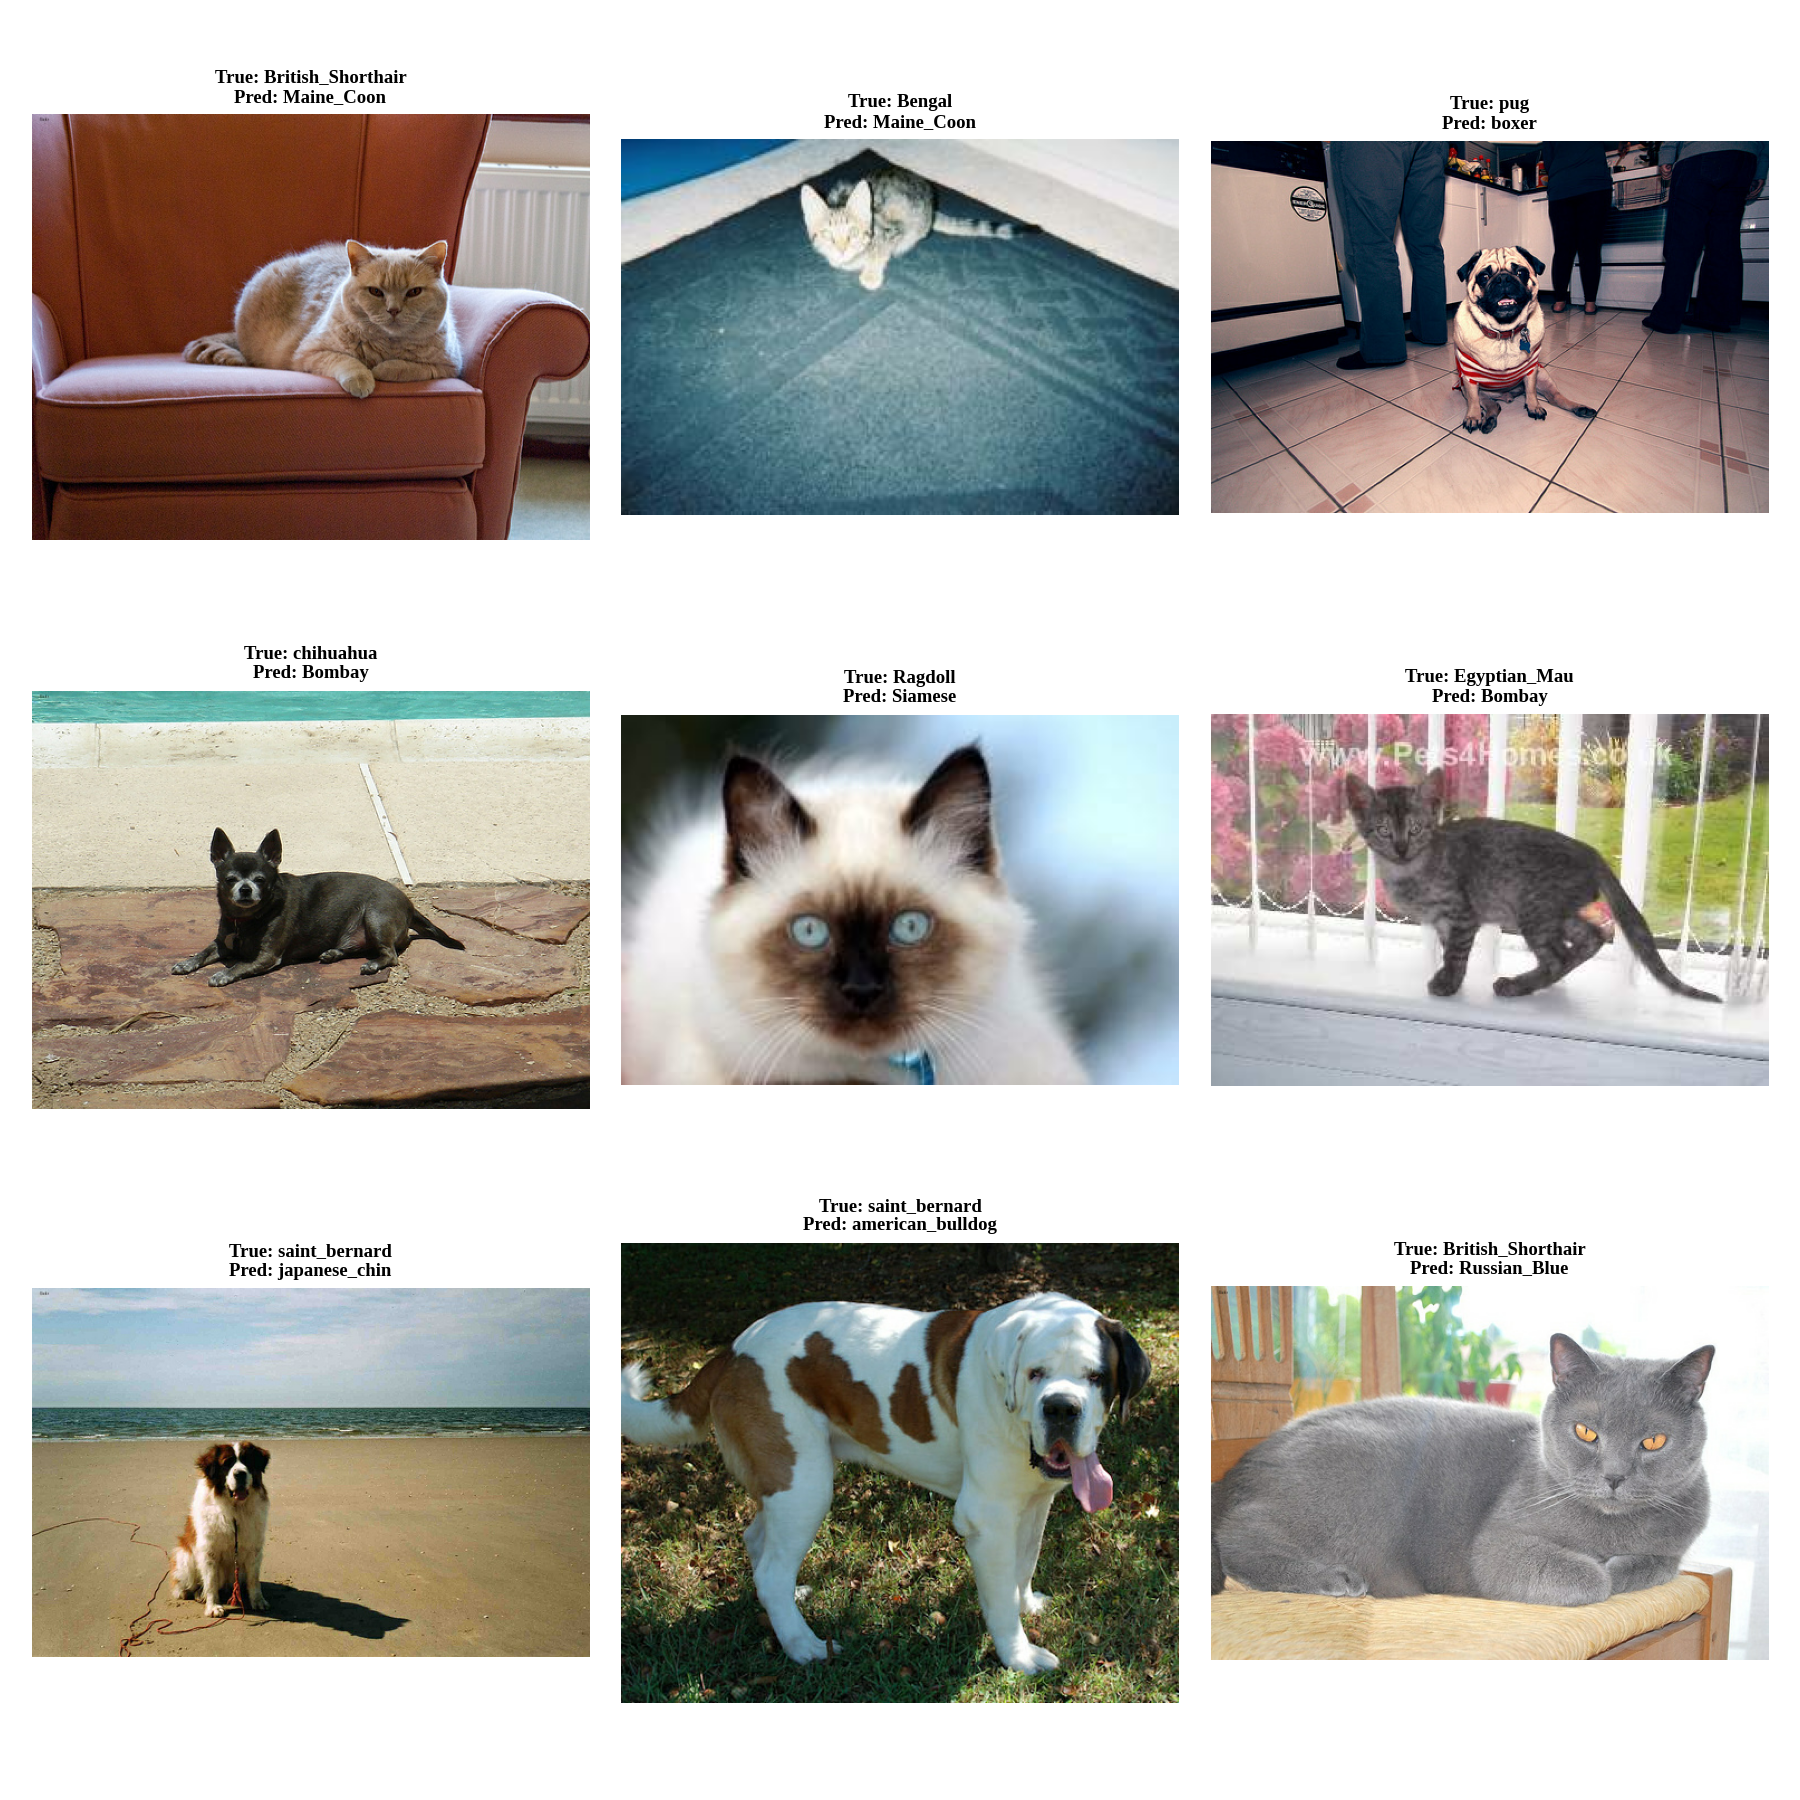
\includegraphics[width=0.75\textwidth]{plots/plot15_misclassified.png}
\end{center}

\textbf{Inference:} The misclassified test images are drawn from the
lowest-accuracy breeds identified above; most errors occur between
breeds with overlapping coat colors/patterns or body shapes at
$224\times224$ resolution, reflecting genuine fine-grained visual
similarity between breeds rather than a systematic model failure.

%%%%%%%%%%%%%%%%%%%%%%%%%%%%%%%%%%%%%%%%%%%%%%%%%%%%%%%%%%%%
\section*{14. Overall Results}

\begin{center}
\begin{tabular}{|l|c|c|c|c|}
\hline
Configuration & CV Accuracy & SD & Test Accuracy & Training Time\\
\hline
Best Initialization (Random)   & -- & -- & -- & 228.05 s\\
Best Regularization (BatchNorm)& -- & -- & -- & 227.81 s\\
Best Optimizer (Adam)          & -- & -- & -- & 227.25 s\\
Best Hyperparameters (C2)      & 0.9114 & 0.0037 & -- & --\\
Fine-Tuned / Final Model       & 0.9114 & 0.0037 & 0.9093 & 155.14 s\\
\hline
\end{tabular}
\end{center}

Students must justify the final model based on accuracy, cross-validation
variability, computational cost and generalization: the final model
(C2, fully-frozen ImageNet base, lr $10^{-3}$, dropout 0.25) was chosen
not for having the single highest raw CV mean (C2 and C3 were within
0.0006 of each other) but for combining a top-tier mean accuracy with the
lowest fold-to-fold variability of the four candidates, and it trained
faster (155.14 s for the full final retrain) than any of the from-scratch
trend-experiment baselines above (which needed 227--228 s just for a
15-epoch run on a much smaller subset) while achieving a test accuracy
(90.93\%) closely matching its cross-validation estimate (91.14\%),
indicating the CV procedure generalized well to the held-out test set.

%%%%%%%%%%%%%%%%%%%%%%%%%%%%%%%%%%%%%%%%%%%%%%%%%%%%%%%%%%%%
\section*{15. Required Inference for Plots}

For every major plot, students must write a short inference containing:

\begin{enumerate}
\item What does the plot show?
\item What trend is observed?
\item Why might the observed trend occur?
\end{enumerate}

Each inference should be approximately 2--3 lines. (See the inference
paragraphs accompanying each plot above, Sections 6--13.)

%%%%%%%%%%%%%%%%%%%%%%%%%%%%%%%%%%%%%%%%%%%%%%%%%%%%%%%%%%%%
\section*{16. Discussion Questions}

\begin{enumerate}

\item \textbf{Model parameters vs.\ hyperparameters:} Parameters
(weights, biases) are learned automatically from data during training via
backpropagation. Hyperparameters (learning rate, batch size, number of
layers, dropout rate) are set by the practitioner before training and
control how learning happens.

\item \textbf{Why is weight initialization important?} It sets the
starting point of optimization. Poor initialization can cause
vanishing/exploding activations or gradients, slow or unstable
convergence, or the network getting stuck in a poor region of the loss
landscape.

\item \textbf{Why can zero initialization be problematic?} All neurons in
a layer receive identical inputs and identical gradients, so they update
identically throughout training (the ``symmetry problem'') -- the layer
effectively behaves like a single neuron no matter how wide it is.

\item \textbf{Xavier vs.\ He initialization:} Xavier/Glorot scales weight
variance by $1/fan_{avg}$ and assumes roughly linear/symmetric activations
(e.g.\ tanh, sigmoid). He scales by $2/fan_{in}$ and is designed for
ReLU-family activations, which zero out roughly half their inputs, so it
compensates with a larger variance to keep signal strength stable.

\item \textbf{Identifying overfitting from curves:} If training accuracy
keeps rising (training loss keeps falling) while validation accuracy
plateaus or falls (validation loss rises), the growing gap between the
two indicates the model is memorizing training data rather than
generalizing.

\item \textbf{How Dropout reduces overfitting:} It randomly deactivates a
fraction of neurons on each forward pass, preventing units from
co-adapting/relying on specific other units, which forces the network to
learn more redundant, robust features. It also approximates ensembling
many sub-networks.

\item \textbf{Purpose of Batch Normalization:} Normalizes layer
activations within each mini-batch to stabilize their distribution during
training, which allows higher learning rates, speeds convergence, and
provides a mild regularizing effect.

\item \textbf{The numerical BN example:} For $x=[2,4,6,8]$, mean$=5$ and
variance$=5$, giving standardized values $[-1.342,-0.447,0.447,1.342]$;
with $\gamma=1,\beta=0$ these are also the final outputs --
approximately zero-centred, unit-scaled activations.

\item \textbf{Roles of $\gamma$ and $\beta$:} They are learnable scale
and shift parameters that let the network undo or adjust the
normalization if the zero-mean/unit-variance distribution isn't actually
optimal for the next layer, preserving representational power.

\item \textbf{SGD vs.\ Momentum vs.\ RMSProp vs.\ Adam:} SGD updates
weights using only the current gradient and can oscillate/converge
slowly. Momentum accumulates a moving average of past gradients to smooth
updates and speed convergence through flat/noisy regions. RMSProp adapts
the learning rate per-parameter using a running average of squared
gradients, helping with ill-conditioned loss surfaces. Adam combines both
ideas (momentum + adaptive per-parameter learning rates), usually giving
fast, stable convergence with less tuning.

\item \textbf{Learning rate too large:} Updates overshoot minima, causing
loss to oscillate, diverge, or fail to converge at all.

\item \textbf{Learning rate too small:} Convergence becomes very slow,
and training may get stuck in poor local minima/saddle points within a
practical epoch budget.

\item \textbf{Effect of increasing batch size:} Gradient estimates become
less noisy (more stable per-step direction) and hardware throughput
improves, but very large batches can generalize slightly worse and
require adjusted learning rates; very small batches are noisier but can
sometimes generalize better.

\item \textbf{Stride and padding:} Stride is the step size the
convolution filter moves across the input (larger stride $\rightarrow$
smaller, coarser output). Padding adds extra pixels (typically zeros)
around the input border so the filter can be applied at edges and to
control output spatial size.

\item \textbf{Why MobileNetV2 is computationally efficient:} It replaces
standard convolutions with depthwise separable convolutions (a
per-channel spatial convolution followed by a $1\times1$ pointwise
convolution), which drastically reduces multiply-add operations, and uses
inverted residuals with linear bottlenecks to keep representations
compact.

\item \textbf{Depthwise separable convolution:} Splits a standard
convolution into two cheaper steps -- a depthwise convolution that
applies one filter per input channel (spatial filtering only), followed
by a pointwise ($1\times1$) convolution that mixes channels -- reducing
computation compared to a single full convolution over all channels
jointly.

\item \textbf{Transfer learning:} Reusing a model (or its learned
features) trained on one task/dataset as the starting point for a
different but related task, instead of training from random
initialization.

\item \textbf{Feature extraction vs.\ fine-tuning:} Feature extraction
freezes the pretrained backbone entirely and only trains a new classifier
head on top of its fixed features. Fine-tuning additionally unfreezes
some (often the later/upper) pretrained layers and continues training
them, usually at a small learning rate, to adapt the learned features to
the new dataset.

\item \textbf{Why fine-tuning uses a smaller learning rate:} The
pretrained weights already encode useful general features; large updates
would overwrite/destroy them rather than gently adapting them, which
would waste the benefit of using a pretrained model in the first place.

\item \textbf{Why K-Fold CV is useful for hyperparameter selection:} It
evaluates each configuration on several different train/validation
splits, giving a more reliable estimate of generalization performance
(mean and variability) than a single split, reducing the risk of
selecting a configuration that only looks good by chance.

\item \textbf{Why the test set must remain untouched during tuning:} If
test performance influences any decisions (model/hyperparameter
selection, early stopping), it stops being an unbiased estimate of
generalization -- the reported result becomes optimistically biased,
since the model was indirectly ``tuned to'' the test set.

\item \textbf{Why report both mean and standard deviation:} Mean alone
hides variability -- two configurations with the same mean CV accuracy
can differ greatly in consistency; SD flags configurations that are
unstable across folds/data splits, which matters for reliability.

\item \textbf{Is highest validation accuracy always sufficient to select
a model?} No -- a model can have high mean accuracy but high variance
across folds (unreliable), be dramatically more expensive to train/run,
or overfit to validation quirks; accuracy should be weighed alongside
variability, computational cost, and how well it's expected to
generalize.

\end{enumerate}

%%%%%%%%%%%%%%%%%%%%%%%%%%%%%%%%%%%%%%%%%%%%%%%%%%%%%%%%%%%%
\section*{17. Additional Exercise}

Two new combinations (from the unused portion of the search space) were
evaluated using the same 5-fold cross-validation procedure and compared
with the originally selected configuration (C2):

\begin{center}
\begin{tabular}{|c|l|c|}
\hline
Config. & Setting & Mean $\pm$ SD\\
\hline
Extra1 & lr $=10^{-4}$, dropout $=0.0$, base fully frozen & $0.8922\pm0.0064$\\
Extra2 & lr $=10^{-3}$, dropout $=0.25$, unfreeze from layer 100 & $0.2519\pm0.0705$\\
\hline
\end{tabular}
\end{center}

\begin{center}
\begin{tabular}{|c|c|c|}
\hline
Configuration & Mean Accuracy & SD\\
\hline
C2 (selected)   & 0.9114 & 0.0037\\
C3              & 0.9108 & 0.0048\\
Extra1          & 0.8922 & 0.0064\\
C1              & 0.8056 & 0.0137\\
C4              & 0.7557 & 0.0111\\
Extra2          & 0.2519 & 0.0705\\
\hline
\end{tabular}
\end{center}

\textbf{Justification:} The originally selected configuration C2 remains
the best choice even after adding the two new candidates -- it has both
the highest mean accuracy and the lowest standard deviation of all six
configurations tested. Extra1 (a lower fixed learning rate, $10^{-4}$,
frozen base) comes closest to C2 but is clearly inferior on both mean
accuracy ($-1.9$ points) and variability (SD $0.0064$ vs.\ $0.0037$).
\textbf{Extra2} is a striking negative result: combining a relatively
large learning rate ($10^{-3}$) with \emph{unfrozen} pretrained layers
caused training to collapse (mean accuracy $0.2519$, barely above the
2.7\% chance level, with a very large SD of $0.0705$ indicating wildly
inconsistent folds). This is a direct, real illustration of Discussion
Question 19: a learning rate appropriate for training a fresh classifier
head is far too large once pretrained convolutional layers are unfrozen,
since large gradient updates destroy the pretrained ImageNet features
before the classifier can make use of them.

%%%%%%%%%%%%%%%%%%%%%%%%%%%%%%%%%%%%%%%%%%%%%%%%%%%%%%%%%%%%
\section*{18. Expected Outcome}

Students should experimentally demonstrate that CNN performance is
strongly influenced by initialization, regularization, optimization and
hyperparameter choices. They should understand the MobileNetV2 architecture,
perform transfer learning and fine-tuning, and select a reliable final
configuration using 5-fold cross-validation.

In this run, the from-scratch trend experiments (Sections 6--10) mainly
demonstrated \emph{training-dynamics} effects (loss reduction, degree of
overfitting) rather than resolvable validation-accuracy differences,
since 15 epochs on a $\sim$2.8k-image subset is not enough to escape
chance-level accuracy on a 37-class problem from random initialization.
Meaningful, well-separated accuracy only emerged once ImageNet-pretrained
weights and the full dataset were used (Sections 11--13), where the final
selected model reached 90.93\% test accuracy.

%%%%%%%%%%%%%%%%%%%%%%%%%%%%%%%%%%%%%%%%%%%%%%%%%%%%%%%%%%%%
\section*{19. References}

\begin{enumerate}
\item Ian Goodfellow, Yoshua Bengio and Aaron Courville,
\emph{Deep Learning}, MIT Press, 2016.

\item Sergey Ioffe and Christian Szegedy,
``Batch Normalization: Accelerating Deep Network Training by Reducing
Internal Covariate Shift,'' ICML, 2015.

\item Mark Sandler, Andrew Howard, Menglong Zhu, Andrey Zhmoginov and
Liang-Chieh Chen, ``MobileNetV2: Inverted Residuals and Linear
Bottlenecks,'' CVPR, 2018.

\item Omkar M. Parkhi, Andrea Vedaldi, Andrew Zisserman and C. V. Jawahar,
``Cats and Dogs,'' IEEE Conference on Computer Vision and Pattern
Recognition, 2012.

\item TensorFlow Documentation:
\url{https://www.tensorflow.org}

\item Keras Documentation:
\url{https://keras.io}
\end{enumerate}

\end{document}